% !TeX encoding = UTF-8
% !TeX root = V34_TEM.tex
% !TeX spellcheck = de_DE_frami

\section{Durchführung}

\subsection{Vorversuch optische Abbildungen}
Die Funktionsweise und Messmodi eines Elektronenmikroskops lassen sich anschaulich am Modell des Lichtmikroskops zeigen. Als Lichtquelle dient uns ein Laser, dessen Strahl durch eine Aufweitungsoptik aus zwei Linsen $L_1, L_2$ mit Brennweiten $f_1, f_2$ und Abstand $f_1 + f_2$ verbreitert wird. Dabei bündelt $L_1$ den Laserstrahl im Brennpunkt zwischen den Linsen, der als Punktquelle für $L_2$ dient und erneut parallelisiert wird. Gemäß dem Strahlensatz wird der Strahl dabei um den Faktor $\frac{f_2}{f_1}$ aufgeweitet, wodurch ein großer Bereich gleichmäßig ausgeleuchtet werden kann.

Nun werden verschiedene Objekte O durch zwei Linsen (Objektiv $L_3$, Okular $L_4$) auf die Wand $B$ abgebildet. Das Objektiv wird anschließend so verschoben, dass das Beugungsbild von O mit $g = \infty$ abgebildet wird.

\begin{figure}[h]
	\centering
	\def\svgwidth{0.75\textwidth}
	\input{graphics/light.pdf_tex}
	\caption{Zeichnung Lichtmikroskop, Abbildung des Objektes}
	\label{fig:light}
\end{figure}


\subsubsection{Spalte und Gitter}
\enlargethispage{2\baselineskip}

\begin{figure}[p]
	\centering
	\begin{subfigure}[b]{0.49\textwidth}
		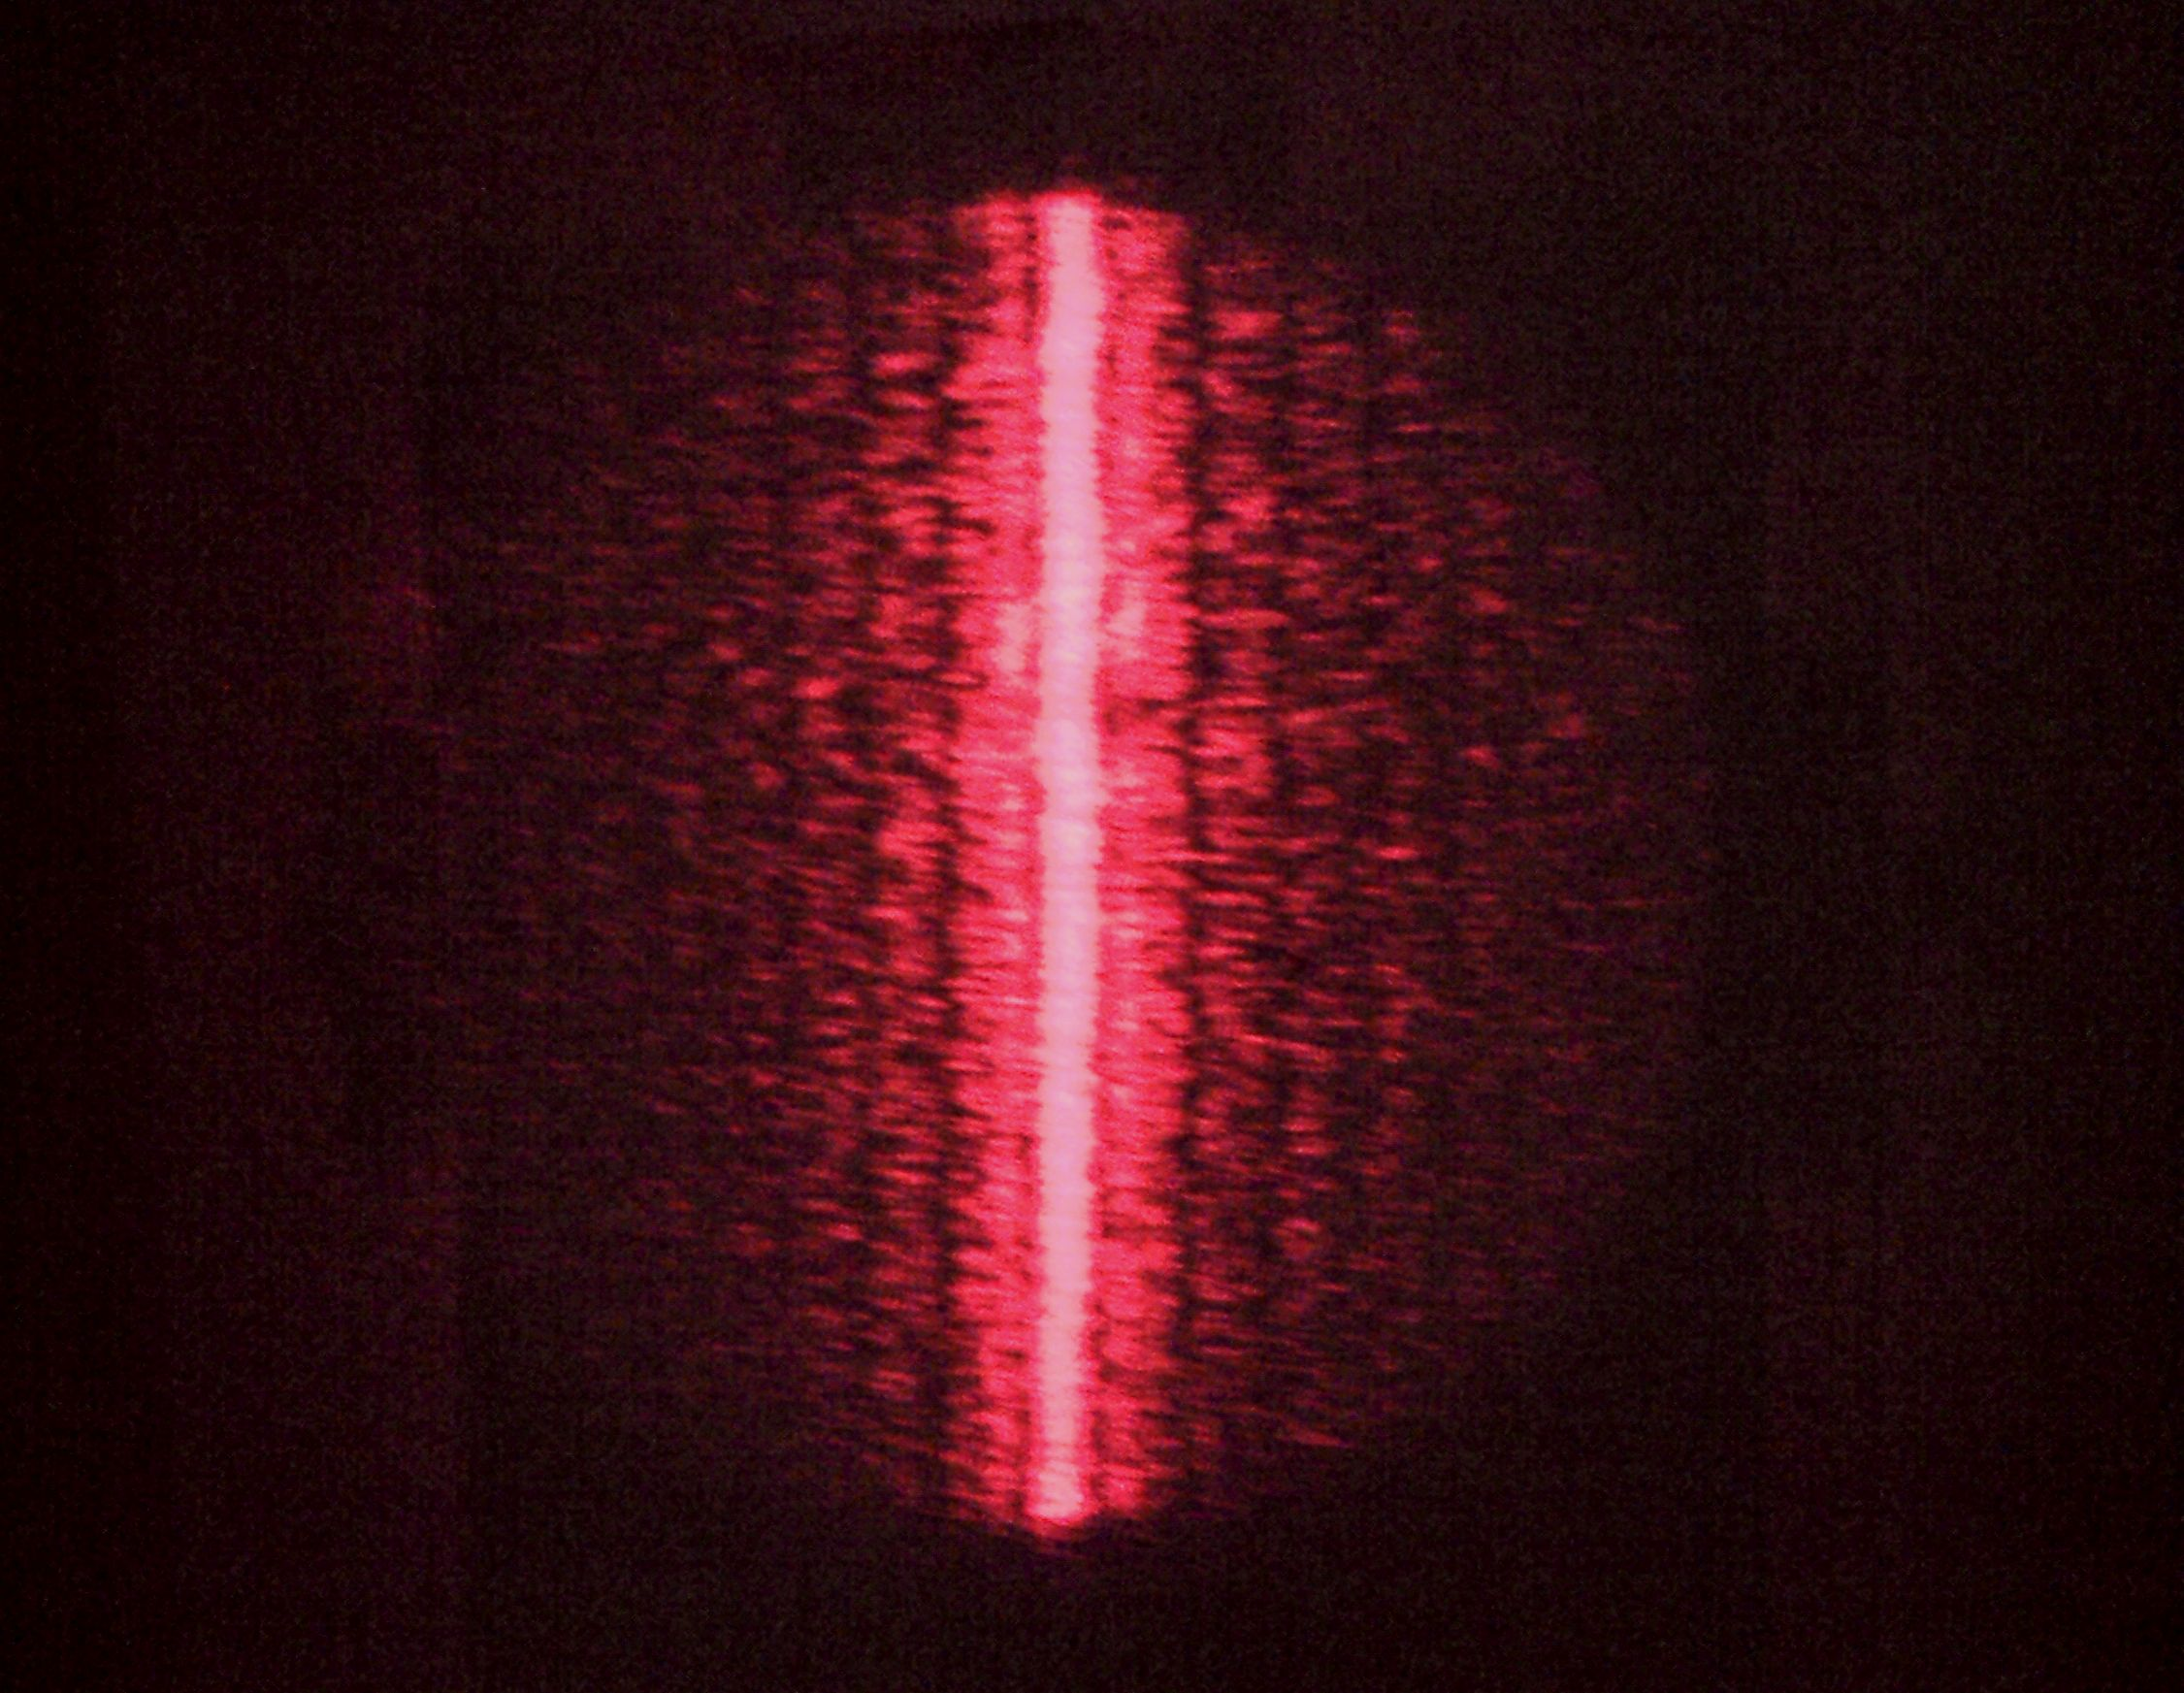
\includegraphics[width=\textwidth]{data/optics/02_Einzelspalt_Bild}
		\caption{Bild}
	\end{subfigure}
	\begin{subfigure}[b]{0.49\textwidth}
		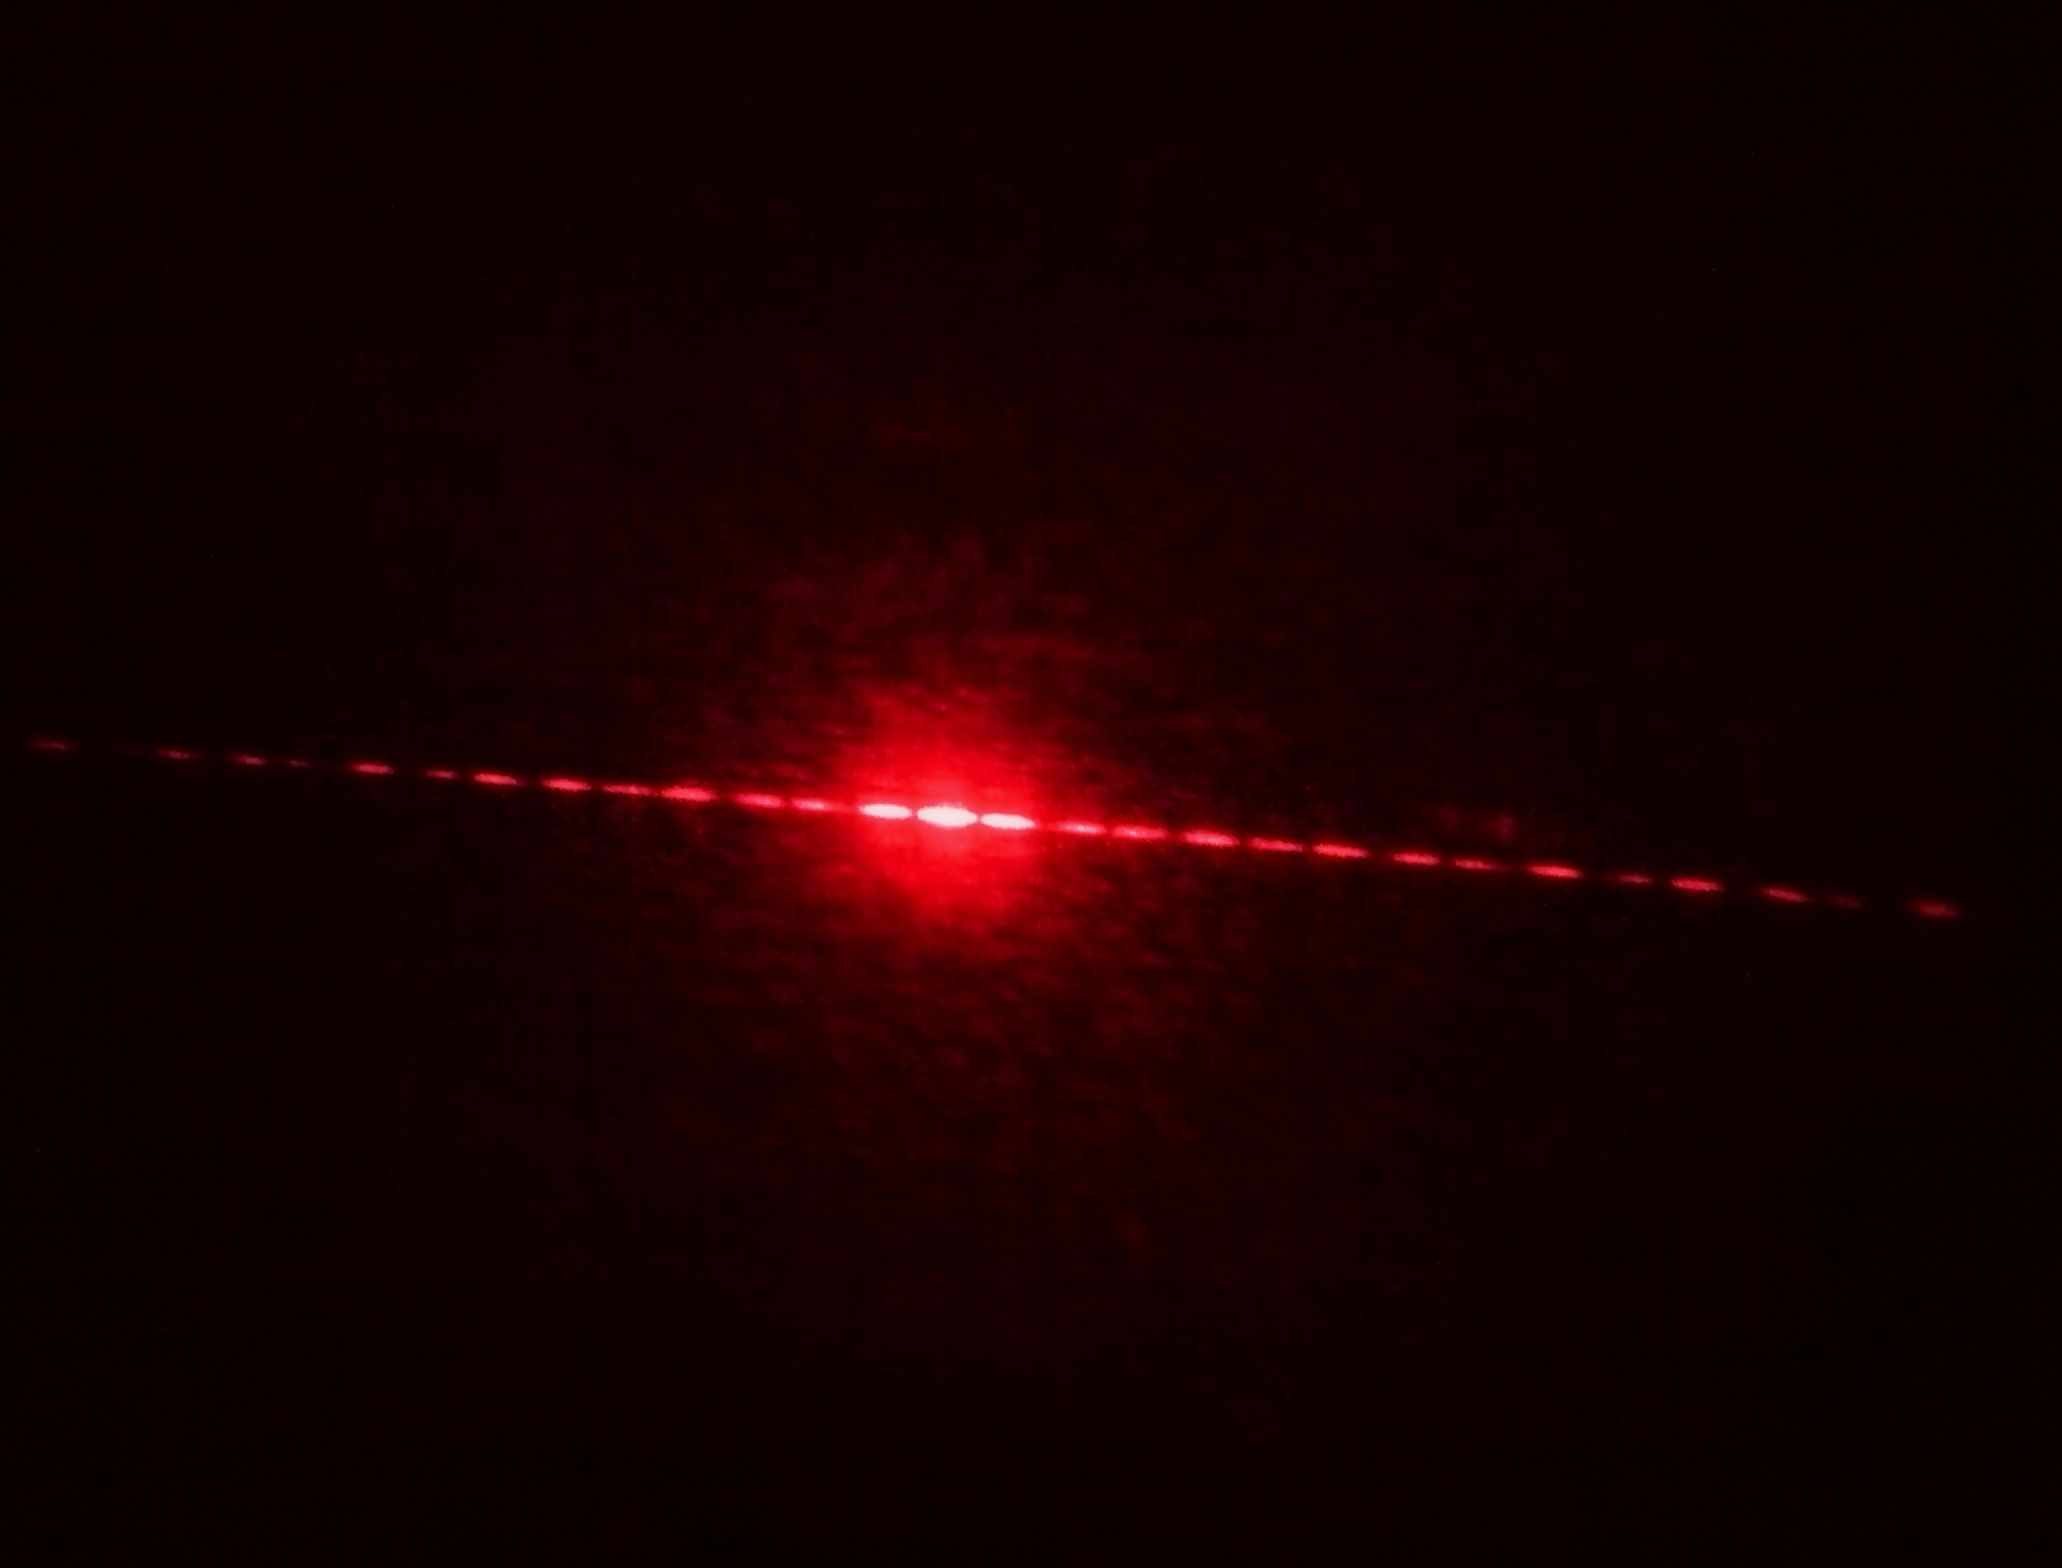
\includegraphics[width=\textwidth]{data/optics/02_Einzelspalt_Beugung}
		\caption{Beugungsbild} 		\label{fig:Einzel_BG}
	\end{subfigure}
	\caption{Einzelspalt}				\label{fig:Einzel}
	\vspace{-1em}
\end{figure}

\begin{figure}[p]
	\centering
	\begin{subfigure}{0.49\textwidth}
		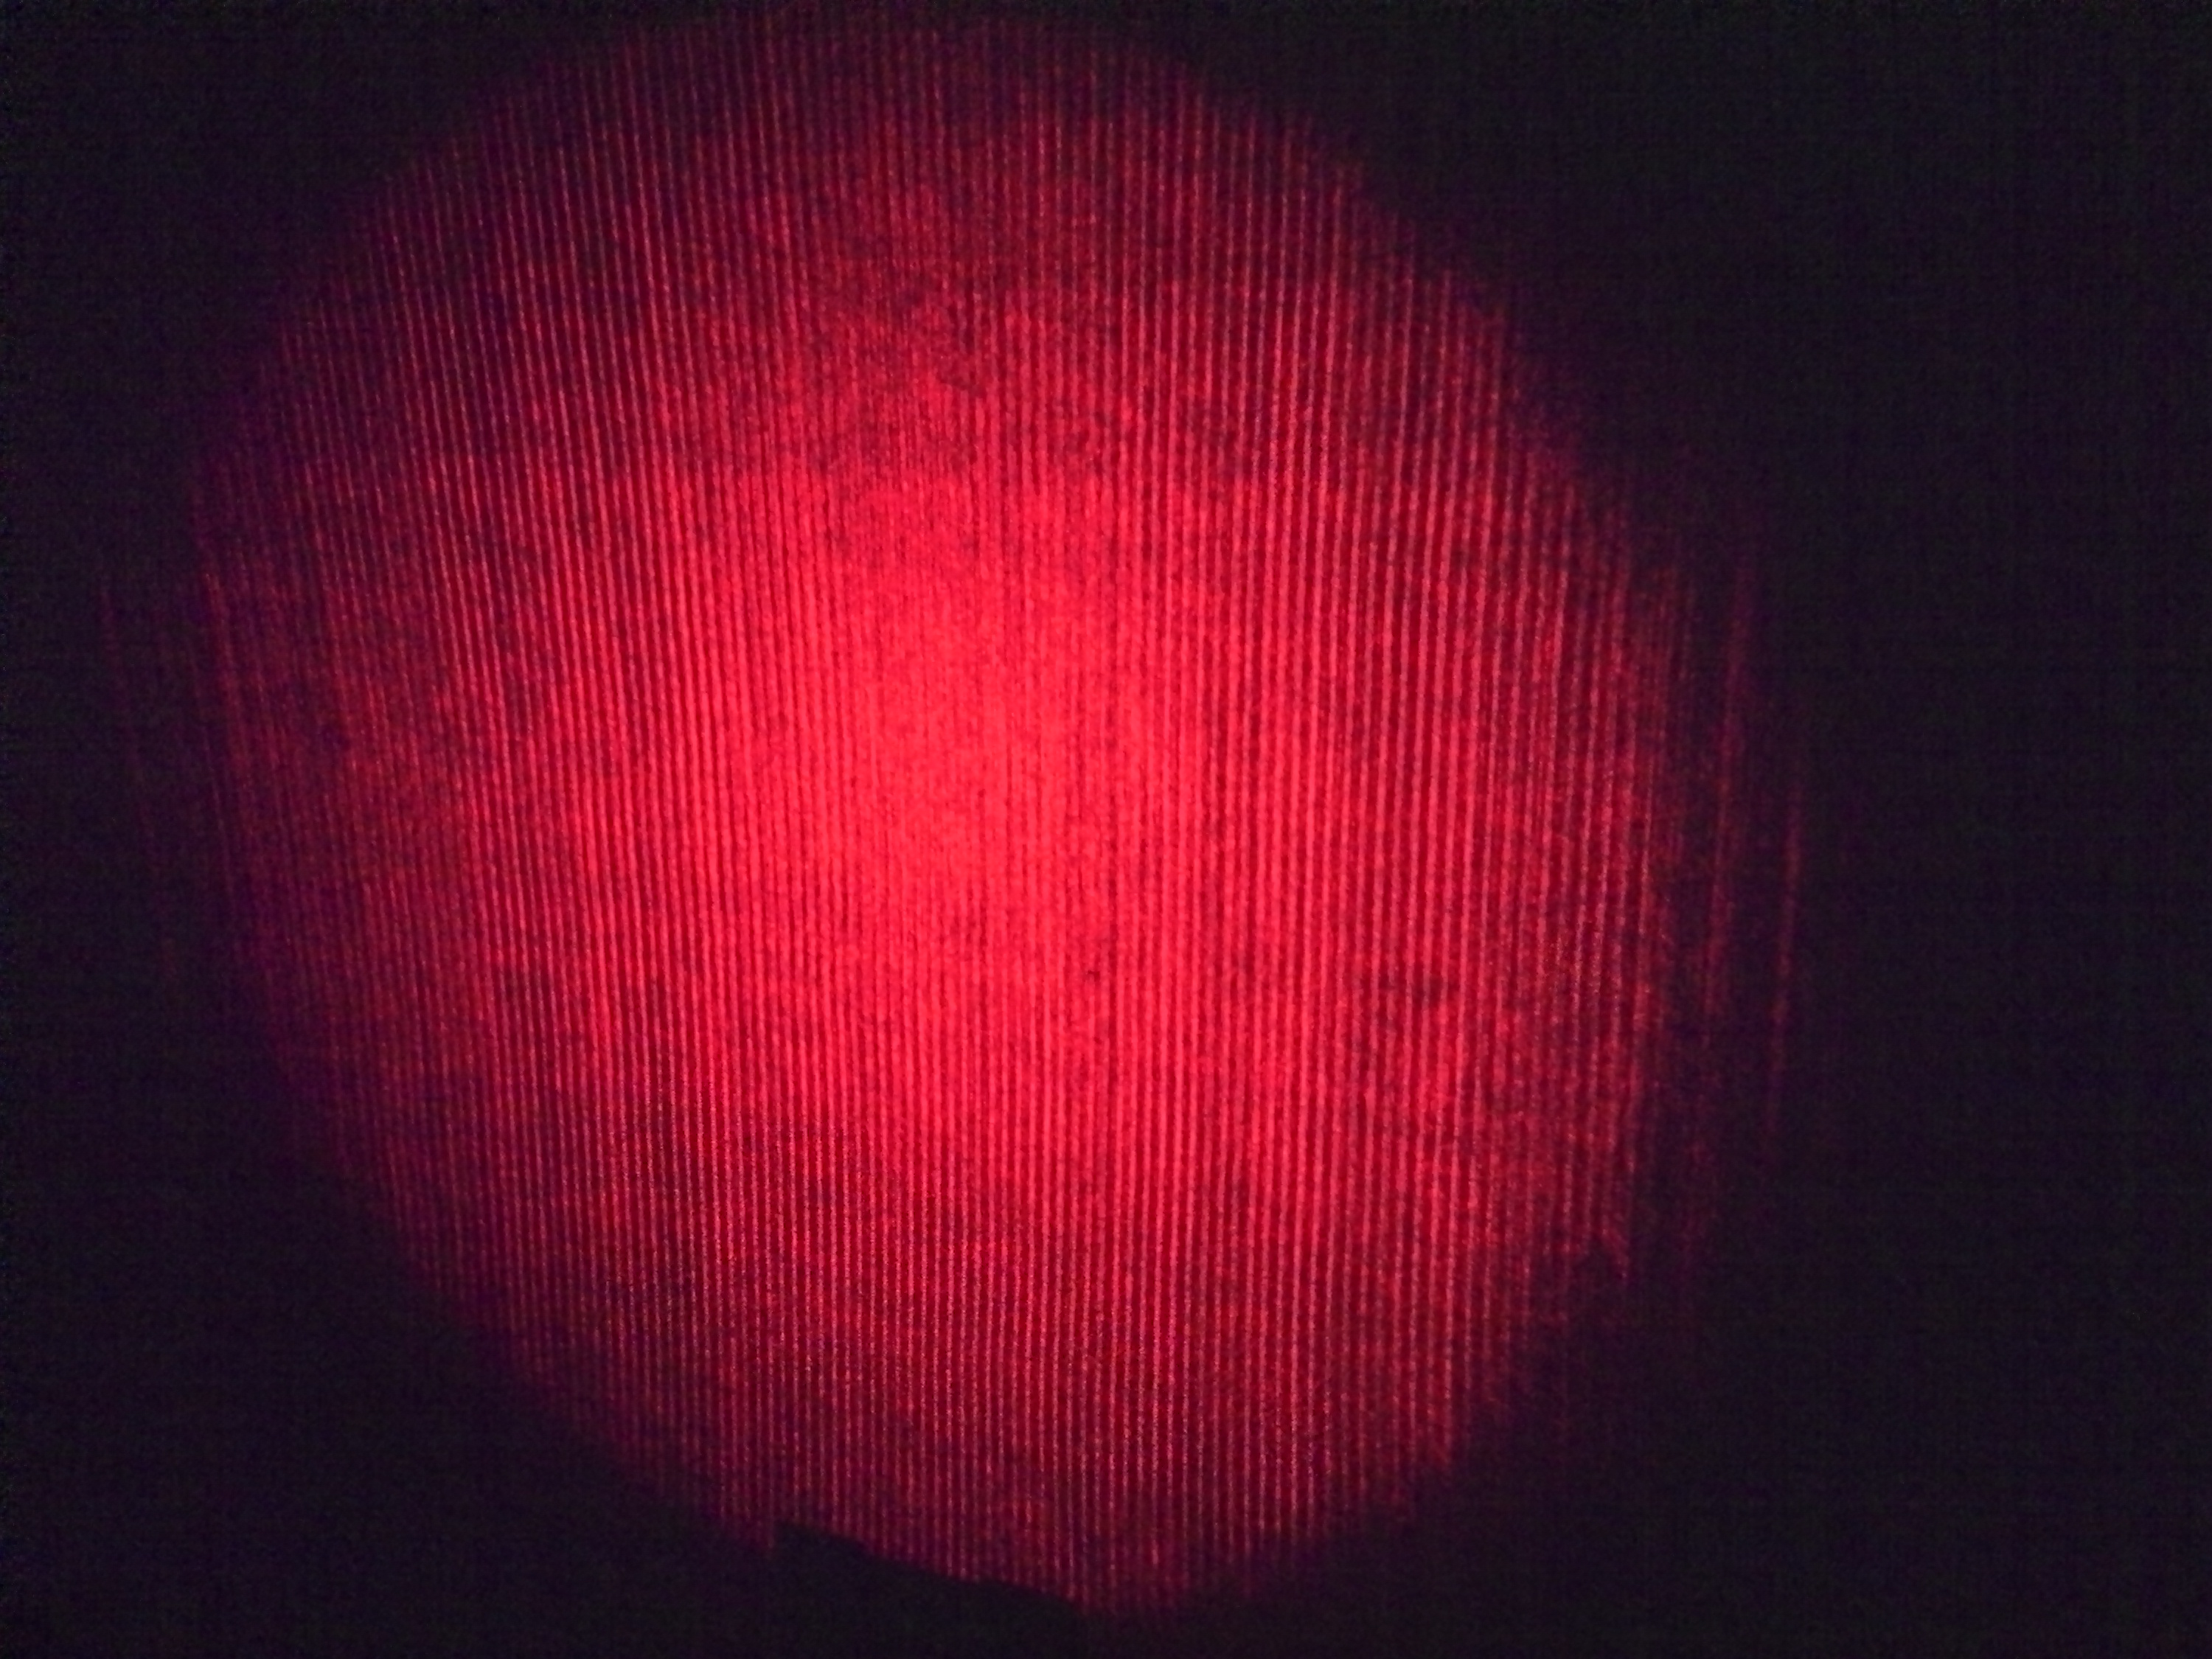
\includegraphics[width=\textwidth]{data/optics/04_Gitter_1D}
		\caption{Bild}
	\end{subfigure}
	\begin{subfigure}{0.49\textwidth}
		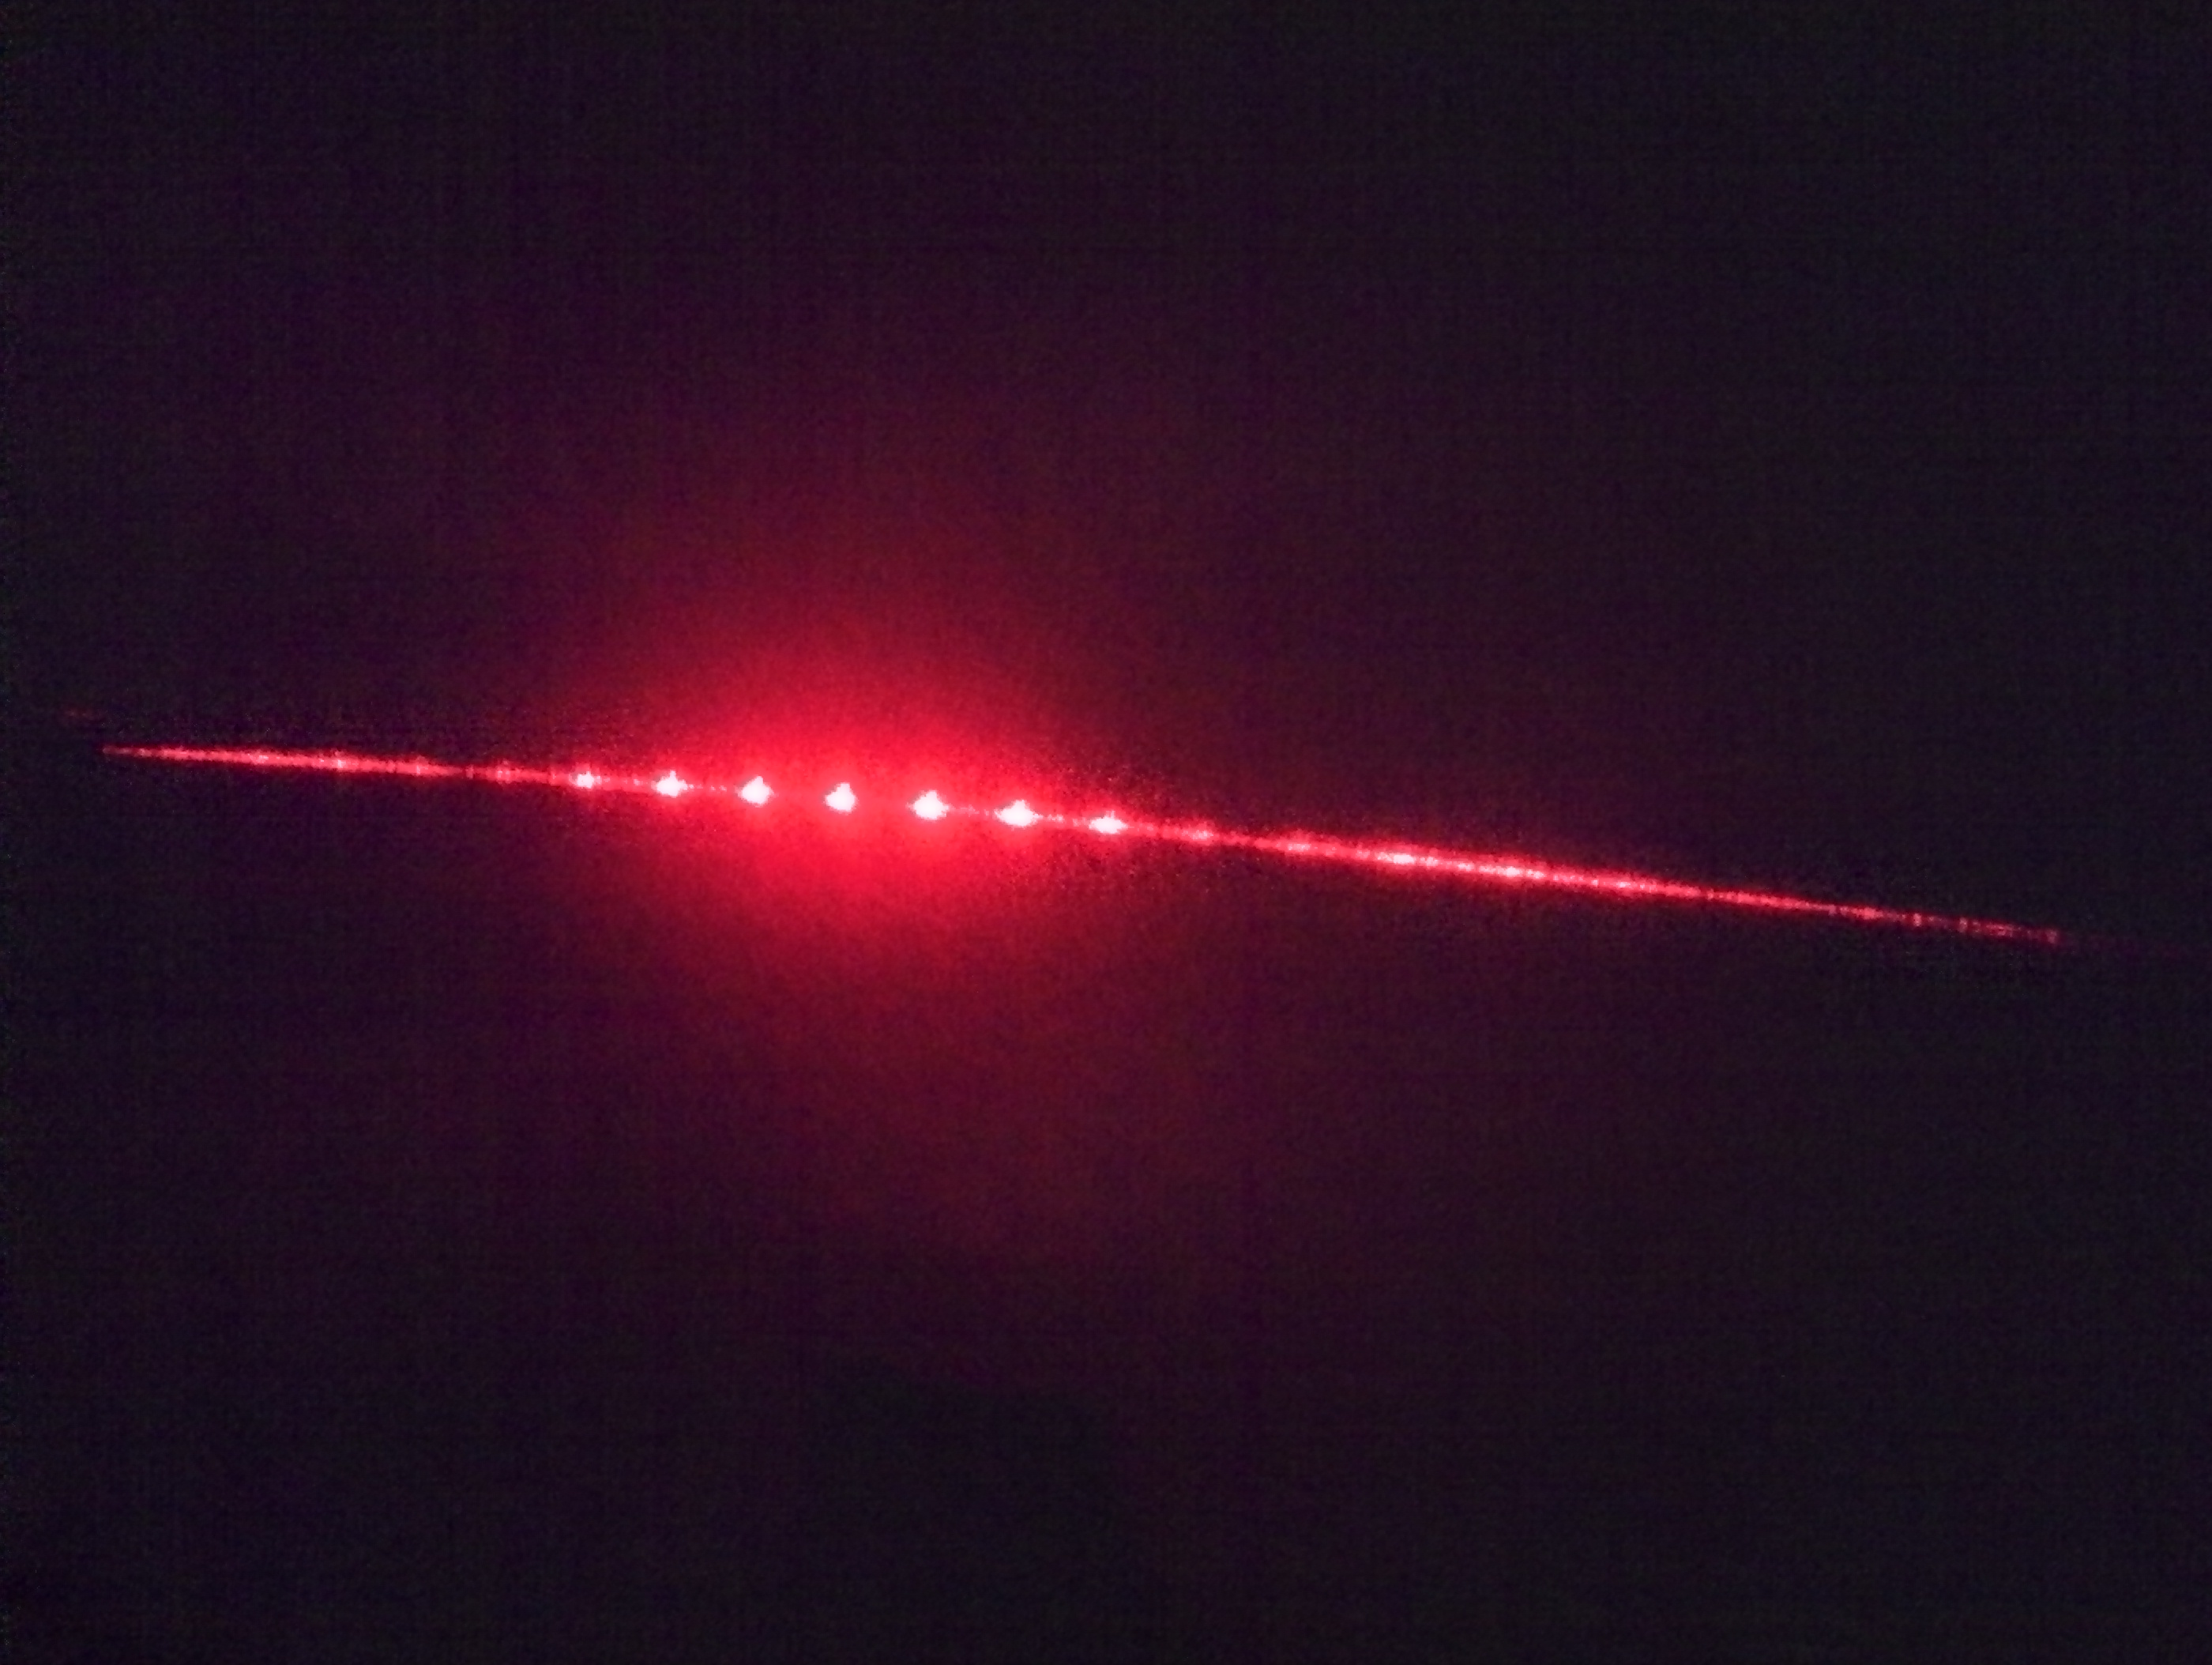
\includegraphics[width=\textwidth]{data/optics/04_Gitter_1D_Beugung}
		\caption{Beugungsbild} 		\label{fig:Gitter_BG}
	\end{subfigure}
	\caption{eindimensionales Gitter}		\label{fig:Gitter}
	\vspace{-1em}
\end{figure}

\begin{figure}[p]
	\centering
	\begin{subfigure}{0.49\textwidth}
		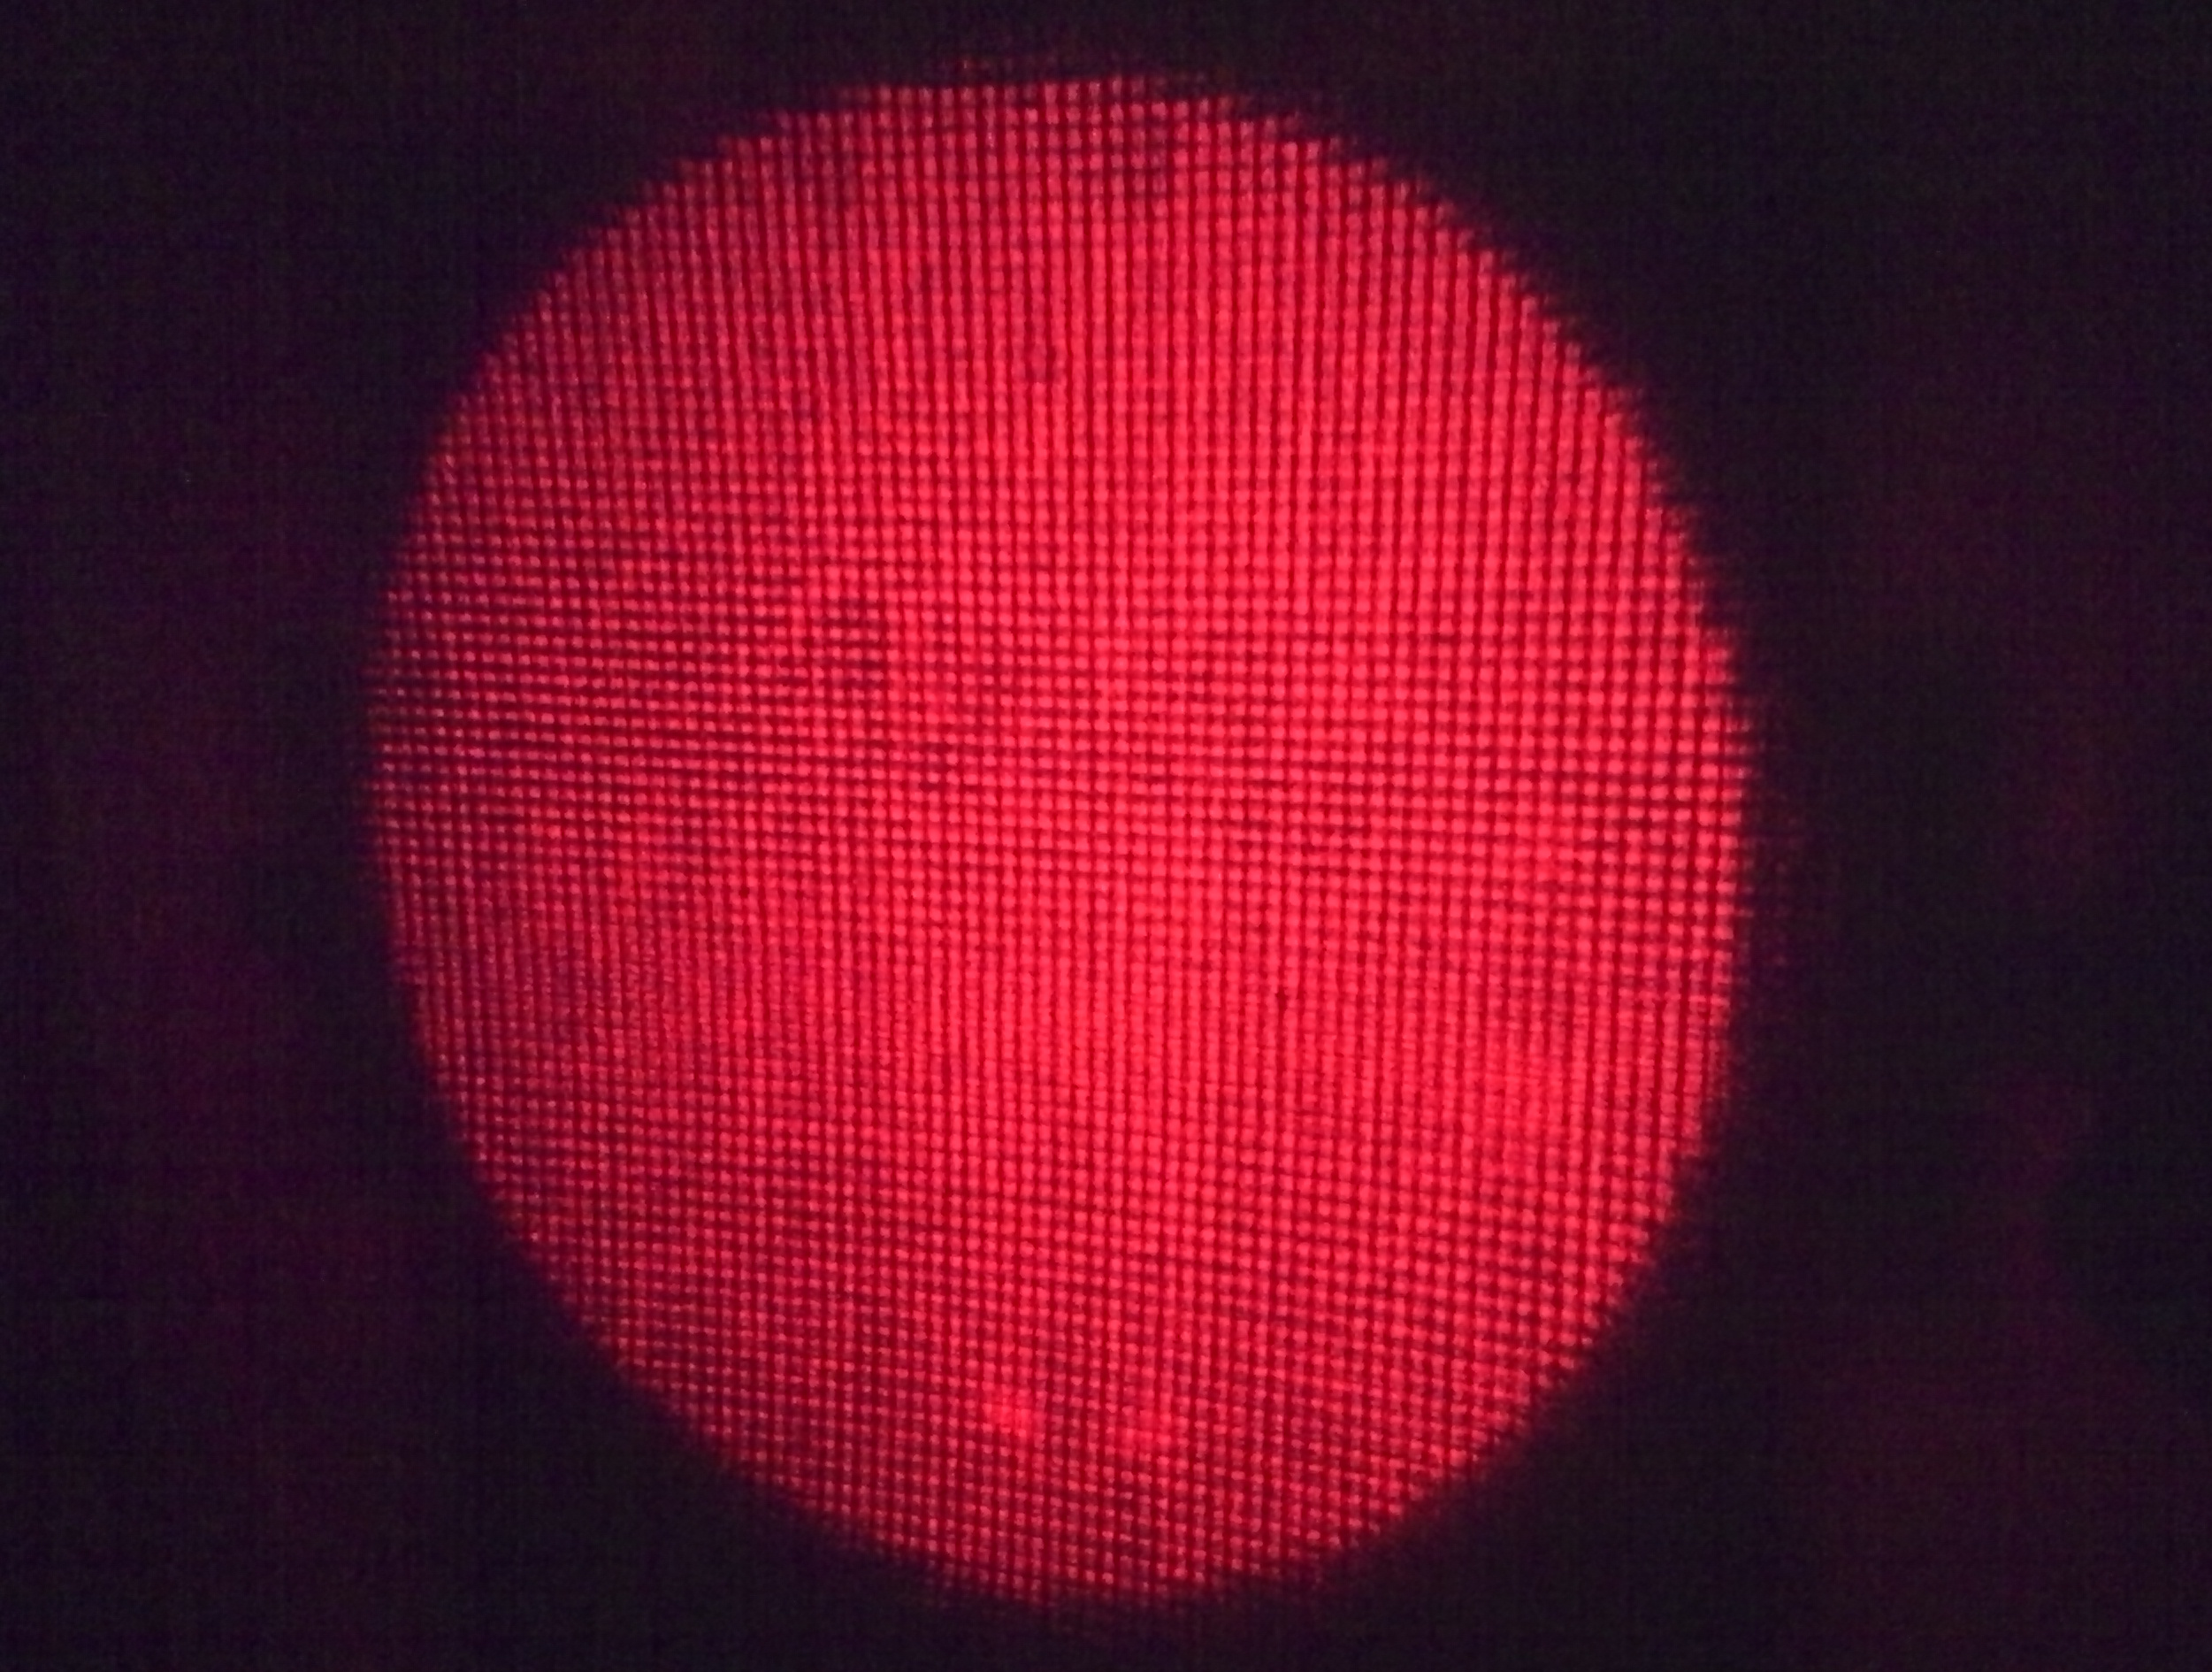
\includegraphics[width=\textwidth]{data/optics/05_Gitter_2D}
		\caption{Bild}
	\end{subfigure}
	\begin{subfigure}{0.49\textwidth}
		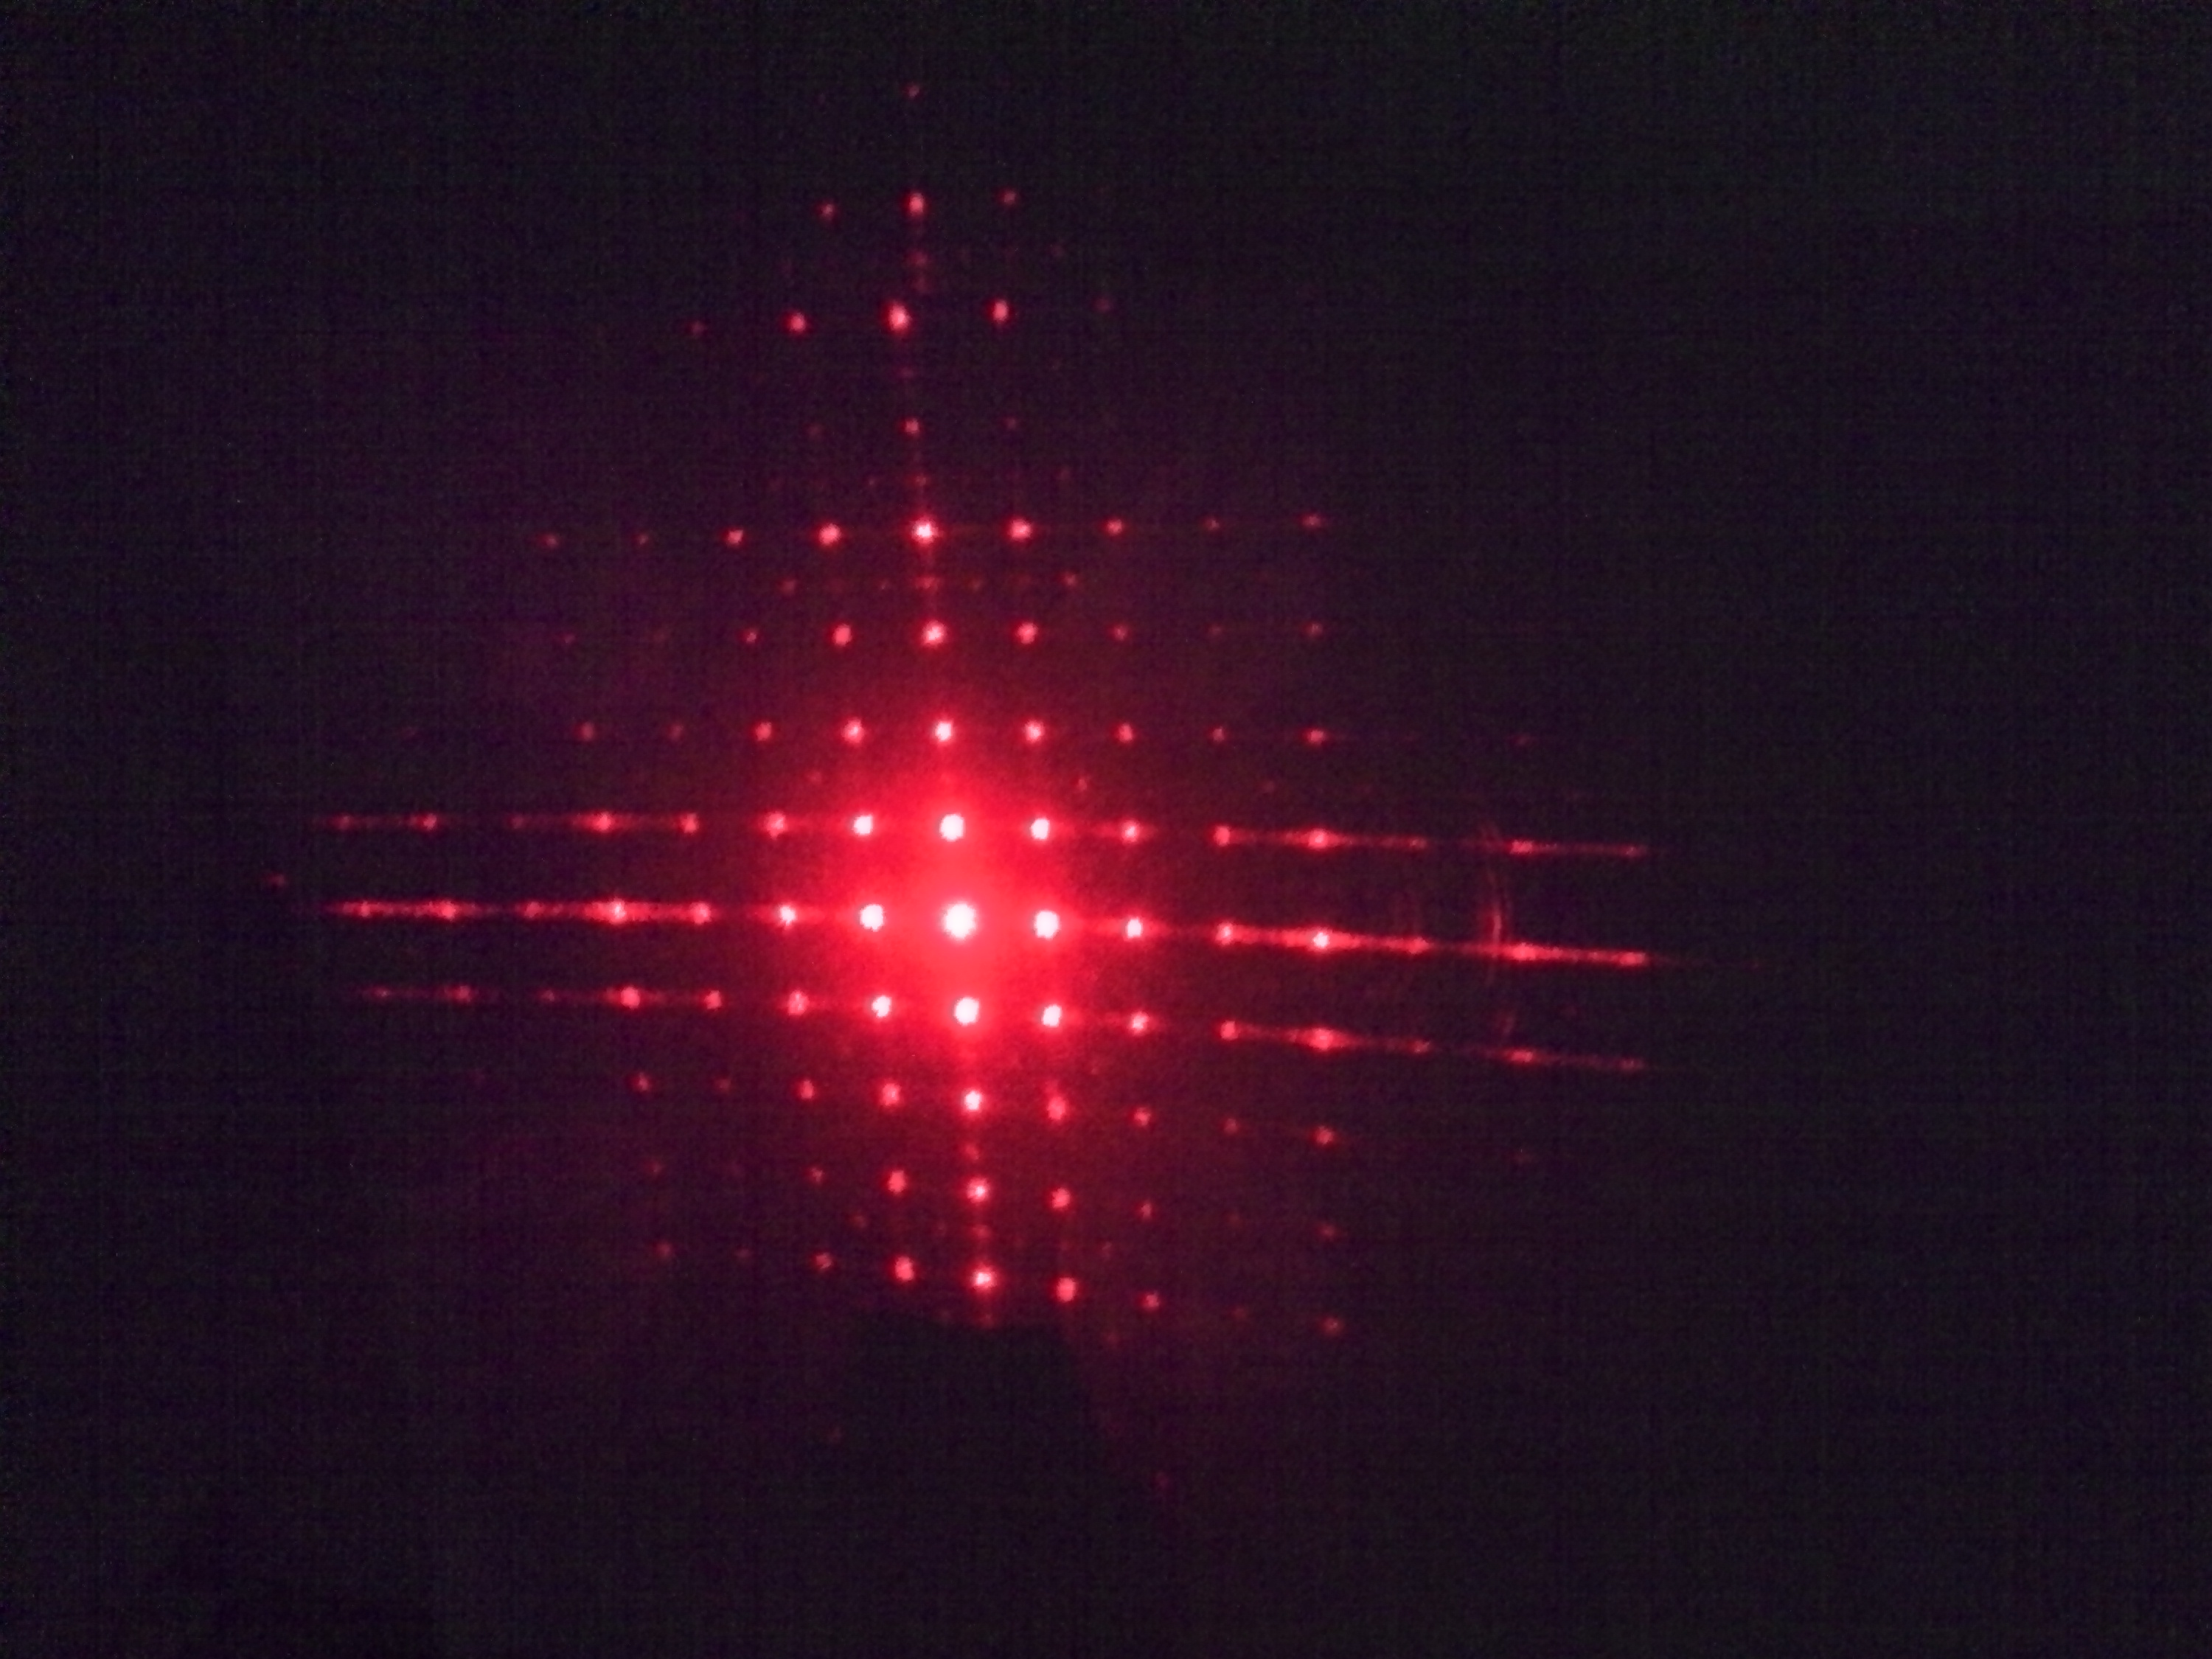
\includegraphics[width=\textwidth]{data/optics/05_Gitter_2D_Beugung}
		\caption{Beugungsbild}		 \label{fig:Gitter_2D_BG}
	\end{subfigure}
	\caption{zweidimensionales Gitter}	\label{fig:Gitter_2D}
	\vspace{-5em}
\end{figure}

Für den Einzelspalt erwarten wir als Intensitätsverlauf im Beugungsbild gemäß Gleichung \eqref{eq:sinc} den Sinus Cardinalis. Das charakteristische Merkmal, das breite Hauptmaximum, ist in unserem Photo jedoch nicht richtig erkennbar (siehe Abb. \ref{fig:Einzel_BG}). Wir vermuten, dass dies am Spalt selbst liegt -- als wir diesen gegen das Licht hielten, war eine schwache zweite Linie erkennbar. Bei einem Doppelspalt wäre das Hauptmaximum gleich breit wie die Nebenmaxima, was das beobachtete Muster erklären würde.

Das Beugungsbild eines perfekten Gitters wäre ein Delta-Kamm, durch die endliche Spaltbreite ist diesem eine $\sinc$-Funktion als Hüllkurve überlagert (Abb. \ref{fig:Gitter_BG}). Da wir den reziproken Raum abbilden, sind kleine Strukturen im Beugungsbild groß und umgekehrt -- da die Spaltbreite deutlich kleiner ist als der Spaltabstand, ist die Hüllkurve breit gegenüber dem Abstand der Maxima.

Das 2D-Gitter ist die Überlagerung zweier 1D-Gitter, somit ist das Beugungsbild ein Punktgitter entlang zweier Achsen (Abb. \ref{fig:Gitter_2D_BG}). Aus diesem ist anhand der gleichen Abstände erkennbar, dass die zwei Gitterkonstanten gleich sind (Netz mit quadratischen Maschen).


\newpage
\subsubsection{Einstein-Portrait}
Auf einem Dia ist das Portrait Einsteins abgebildet, allerdings ist dieses durch ein Gitter überlagert, wodurch man nur ein verschwommenes Bild erhält (Abb. \ref{fig:Einstein_B}). Da das Gitter deutlich feiner ist als das Portrait, zeigen sich im Beugungsbild die typischen Punktreflexe eines Gitters (Abb. \ref{fig:Einstein_BG}). Gemäß dem Faltungstheorem enthält jeder dieser Reflexe die Information des Portraits.

Selektieren wir durch eine Rechteckblende im Brennpunkt von $L_3$ ausschließlich das Hauptmaximum (Abb. \ref{fig:Einstein_hell_B}), so entfällt die Information des Gitters und erhalten ein gefiltertes Bild. Diese Methode wird als Hellfeld-Mikroskopie bezeichnet.

Verschieben wir die Rechteckblende so, dass lediglich das Licht eines Nebenmaximums hindurch gelangt (Abb. \ref{fig:Einstein_dunkel_B}), so sehen wir im Bild nur das am Objekt gestreute Licht und sehen folglich das Portrait auf dunklem Hintergrund, daher auch der Name Dunkelfeld-Mikroskopie. Der Kontrast ist typischerweise besser, allerdings ist die Intensität des gestreuten Lichts verständlicherweise deutlich geringer als im Hellfeld.

\begin{figure}[p]
	\centering
	\begin{subfigure}[b]{0.49\textwidth}
		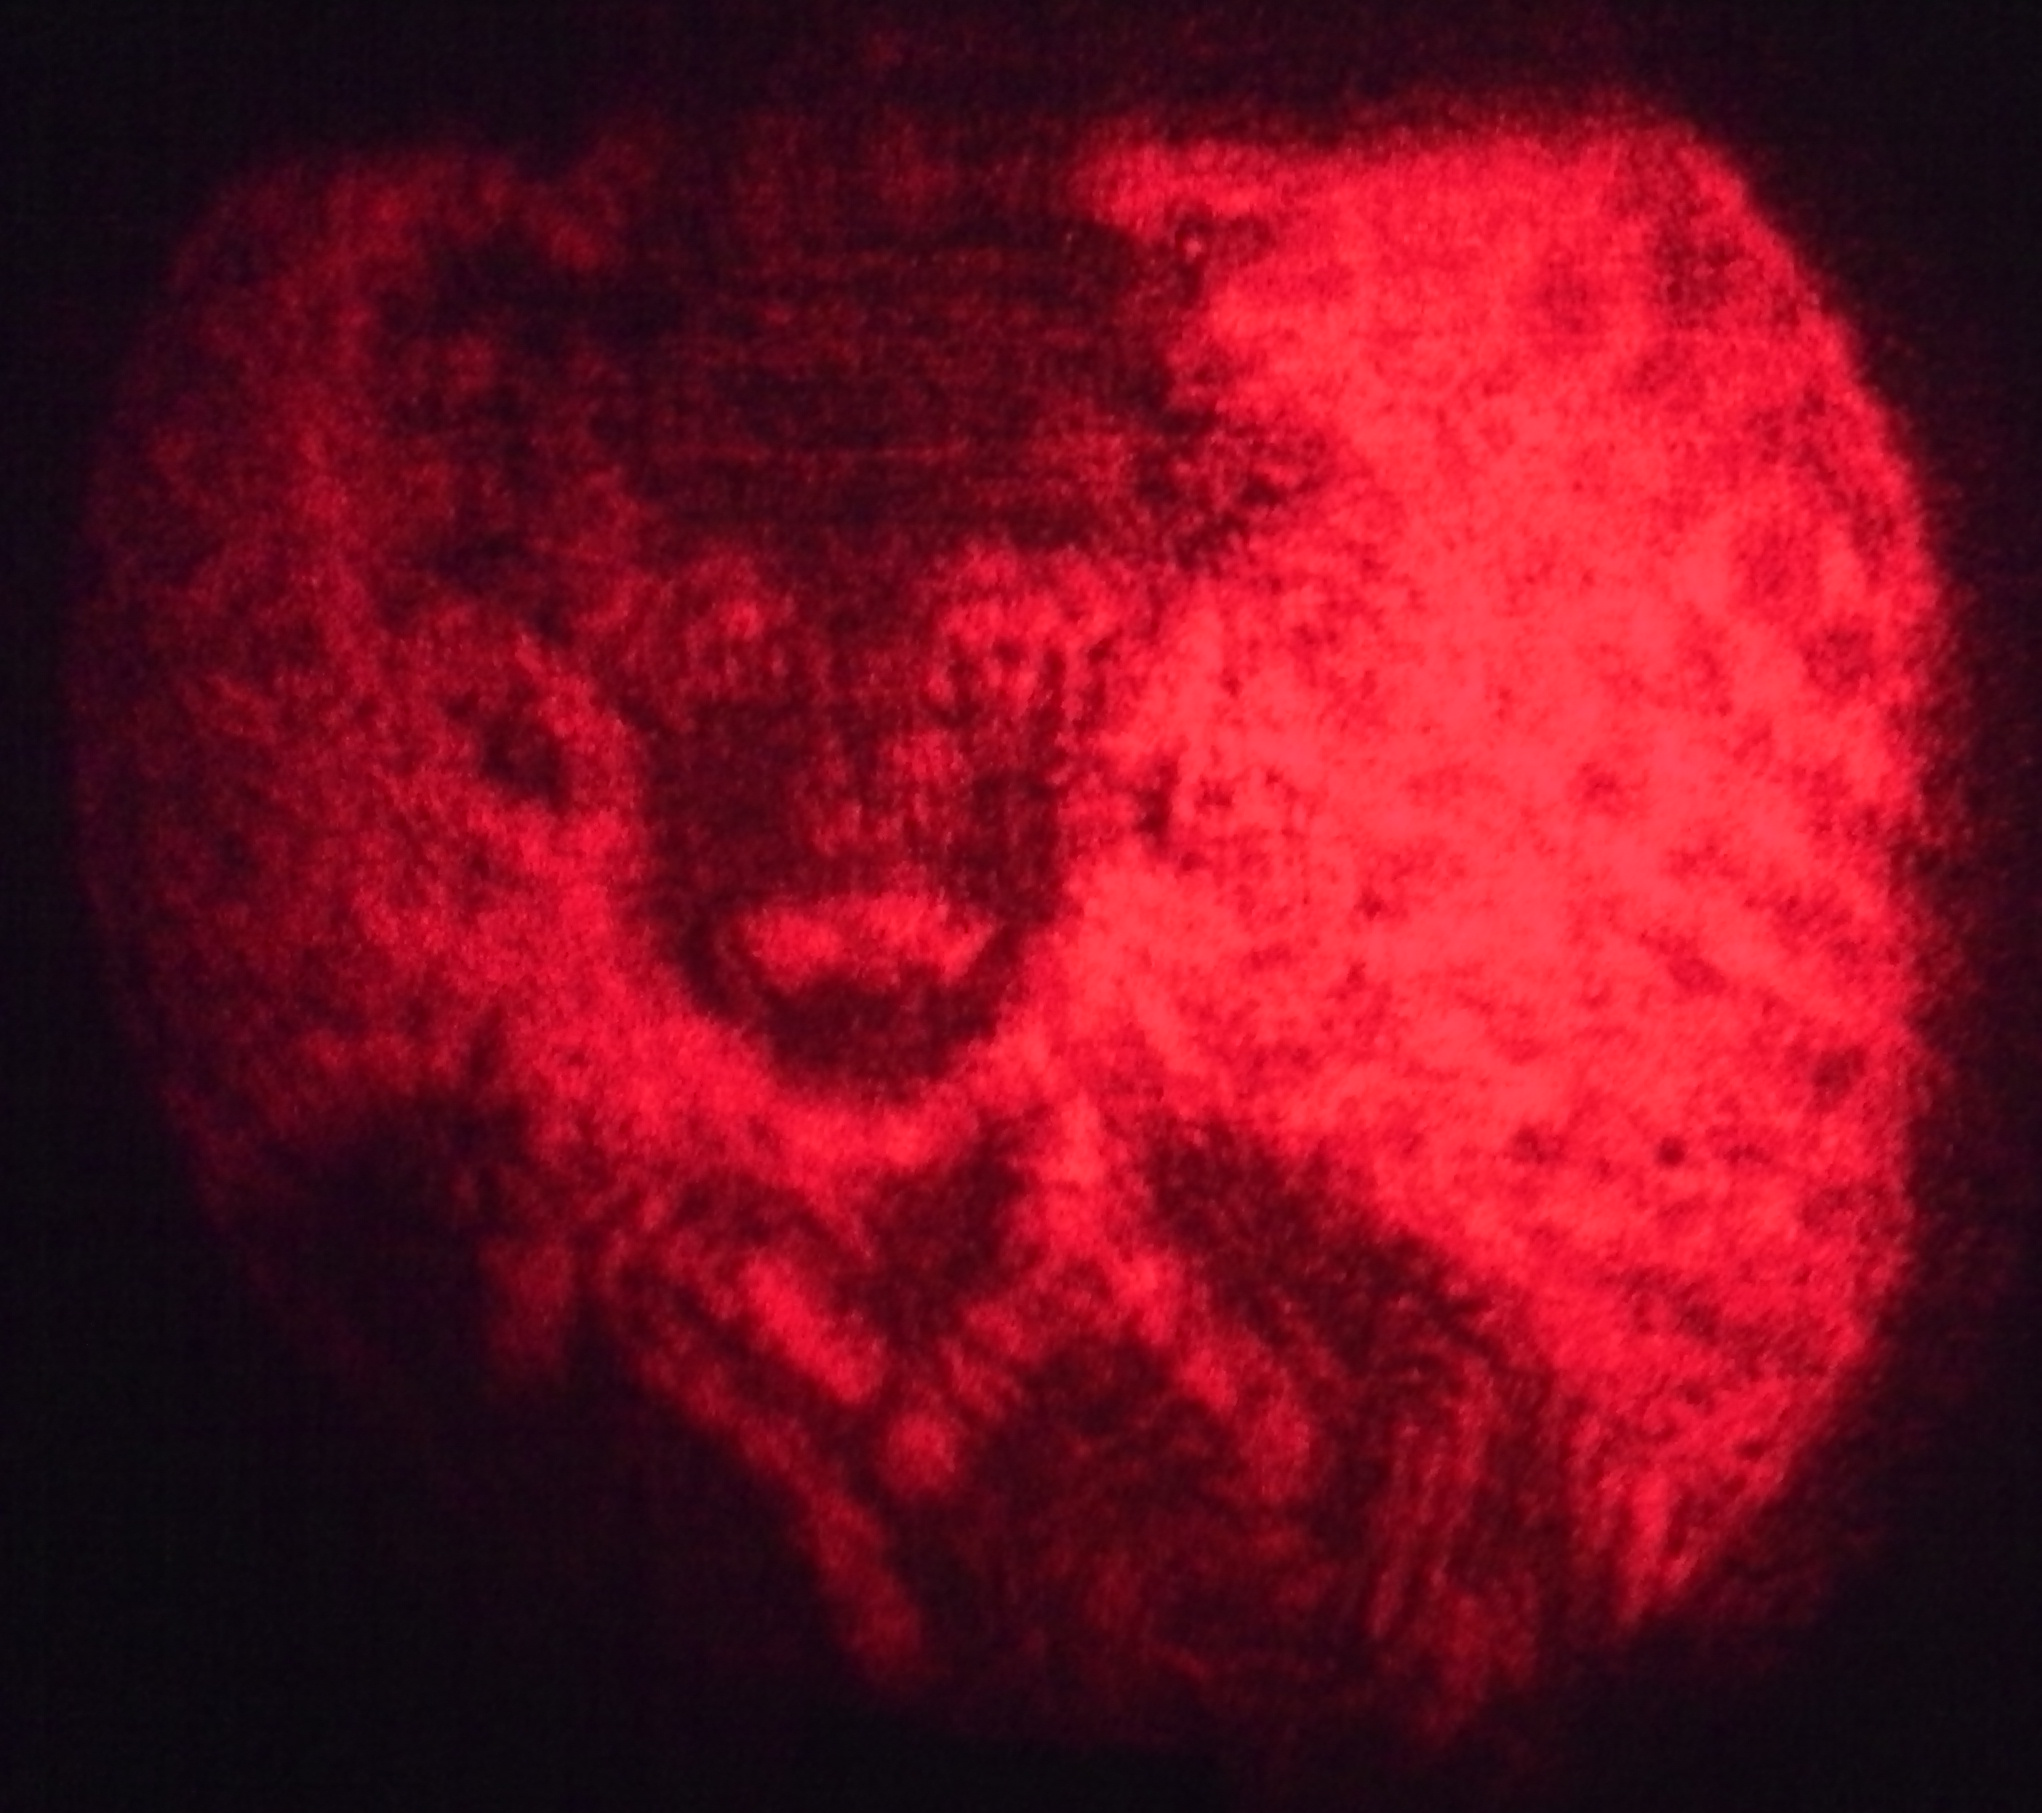
\includegraphics[width=\textwidth]{data/optics/06_Einstein_Bild}
		\caption{Bild}				\label{fig:Einstein_B}
	\end{subfigure}
	\begin{subfigure}[b]{0.49\textwidth}
		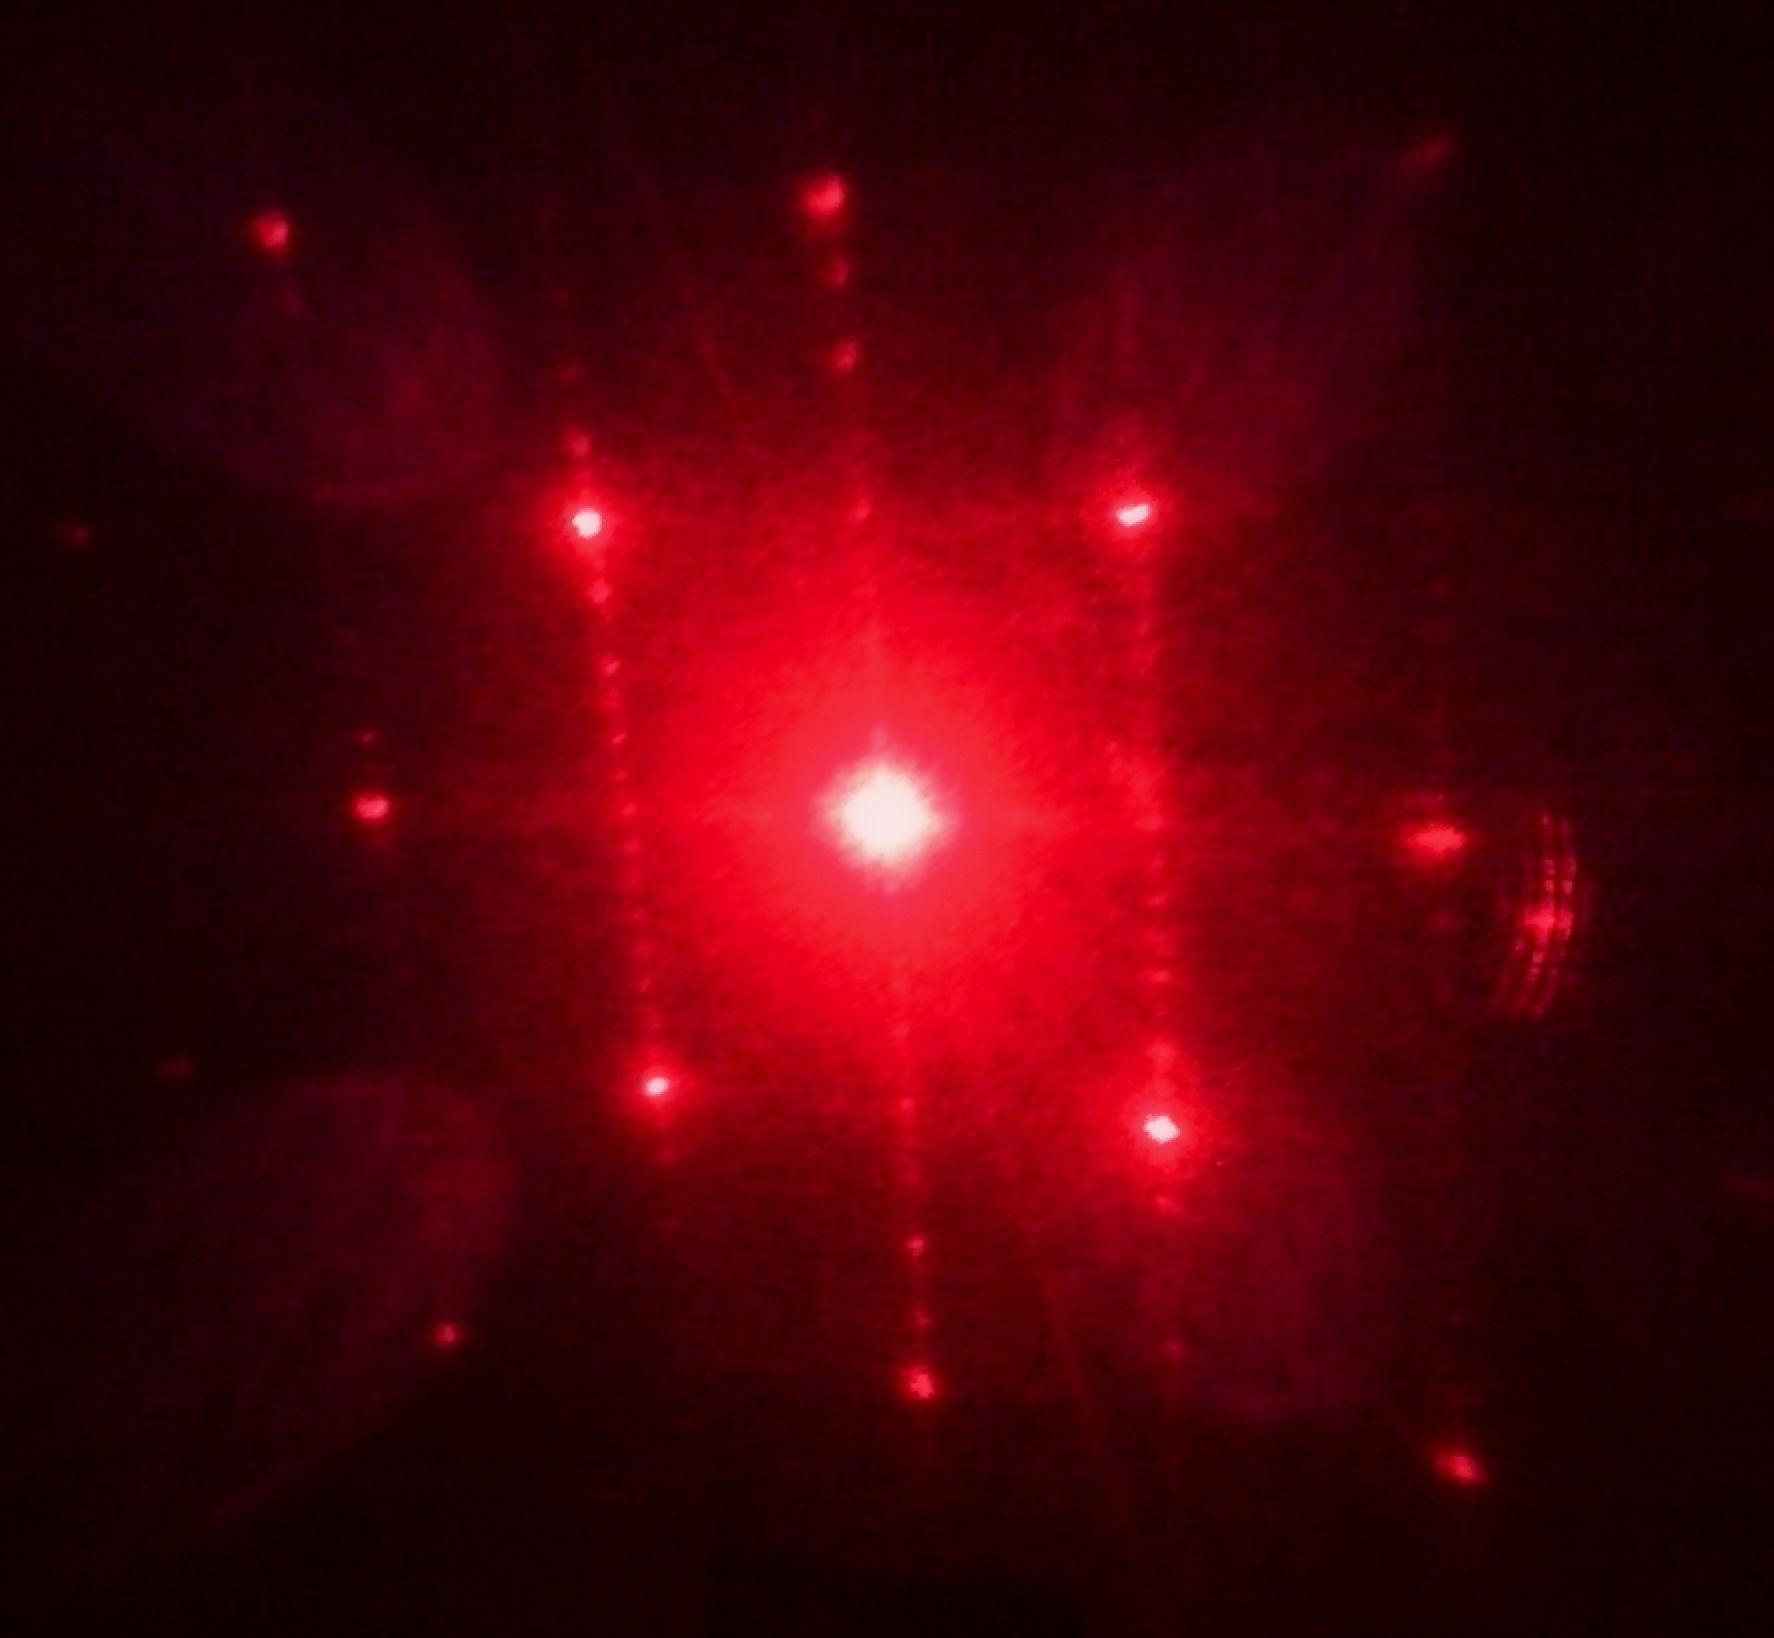
\includegraphics[width=\textwidth]{data/optics/06_Einstein_Beugung}
		\caption{Beugungsbild} 		\label{fig:Einstein_BG}
	\end{subfigure}
	\caption{Einstein-Portrait}			\label{fig:Einstein}
	\vspace{-1em}
\end{figure}

\begin{figure}[p]
	\centering
	\begin{subfigure}{0.49\textwidth}
		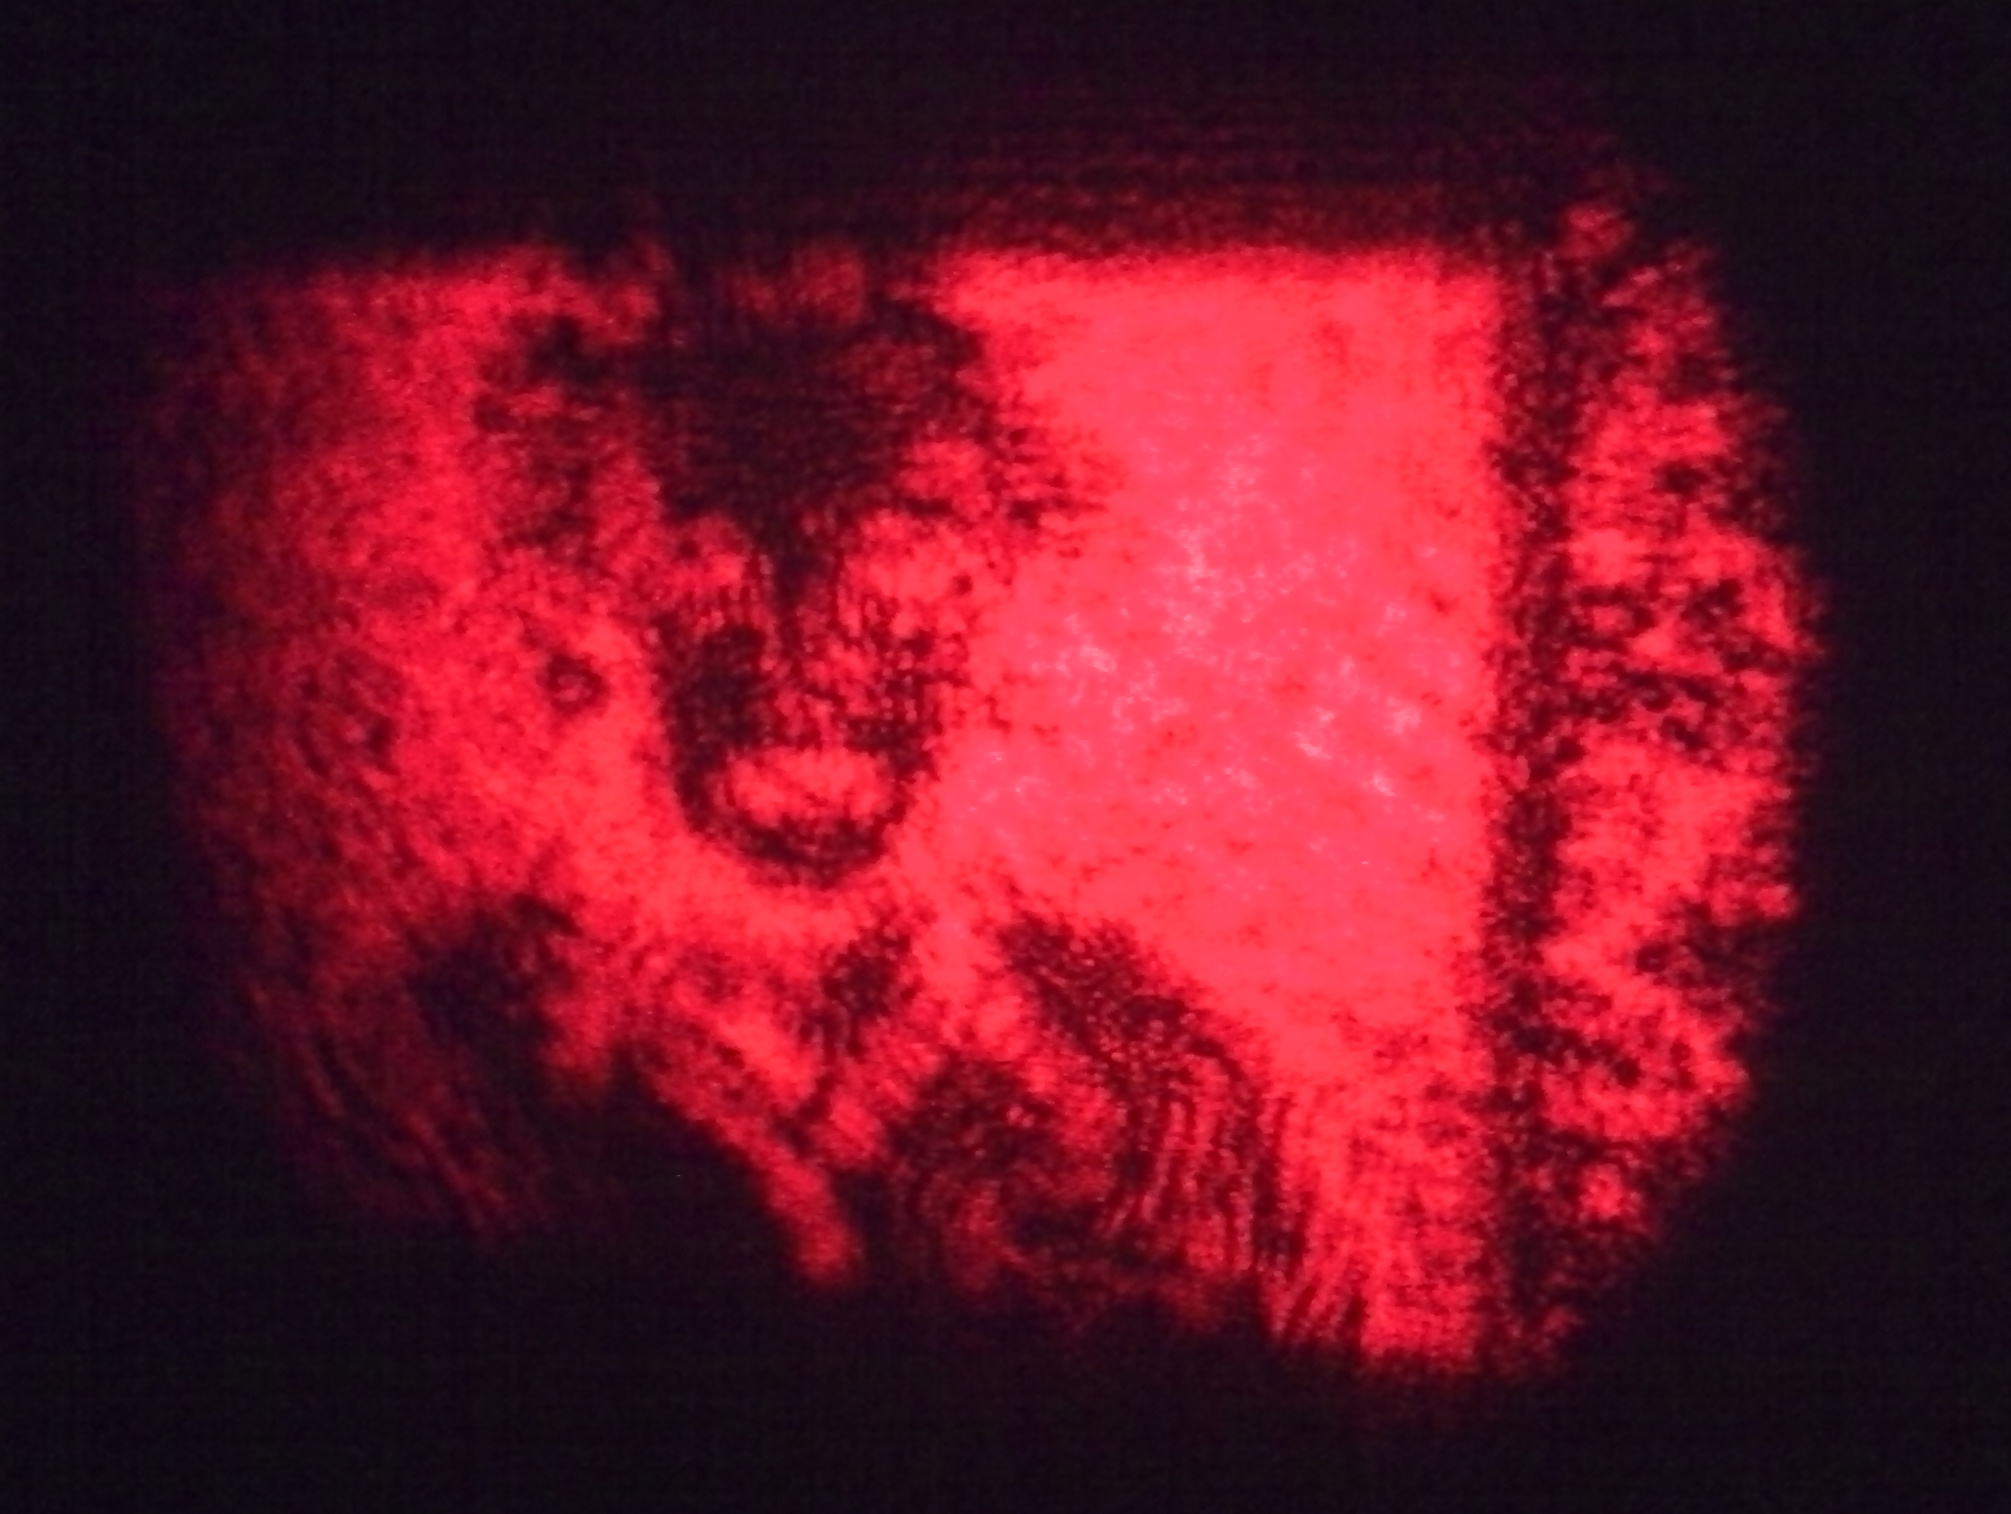
\includegraphics[width=\textwidth]{data/optics/06_Einstein_Hell_Bild}
		\caption{Hellfeld-Bild}				\label{fig:Einstein_hell_B}
	\end{subfigure}
	\begin{subfigure}{0.49\textwidth}
		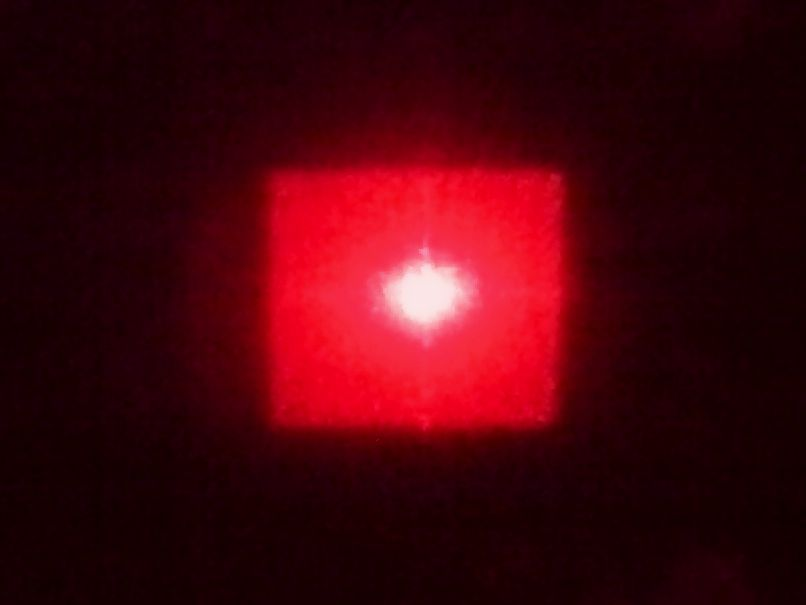
\includegraphics[width=\textwidth]{data/optics/06_Einstein_Hell_Beugung}
		\caption{Beugungsbild: Hauptmaximum}	\label{fig:Einstein_hell_BG}
	\end{subfigure}
	\caption{Einstein-Portrait im Hellfeld}		\label{fig:Einstein_hell}
	\vspace{-1em}
\end{figure}

\begin{figure}[p]
	\centering
	\begin{subfigure}{0.49\textwidth}
		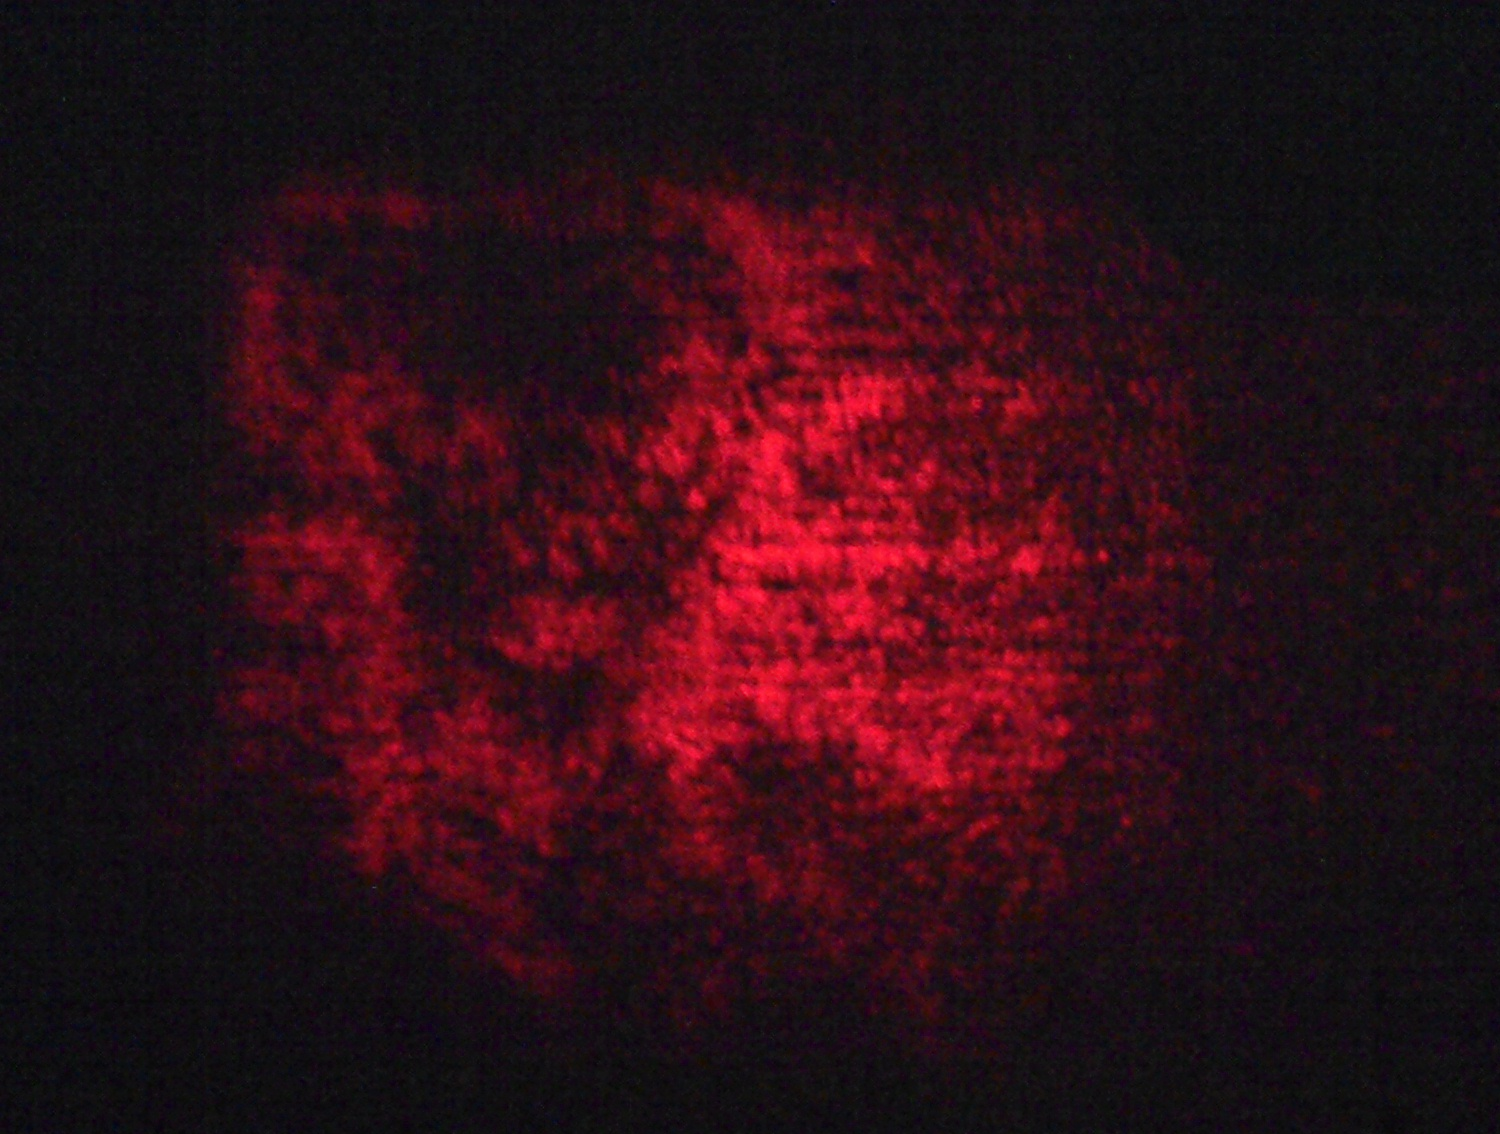
\includegraphics[width=\textwidth]{data/optics/06_Einstein_Dunkel_Bild}
		\caption{Dunkelfeld-Bild}				 \label{fig:Einstein_dunkel_B}
	\end{subfigure}
	\begin{subfigure}{0.49\textwidth}
		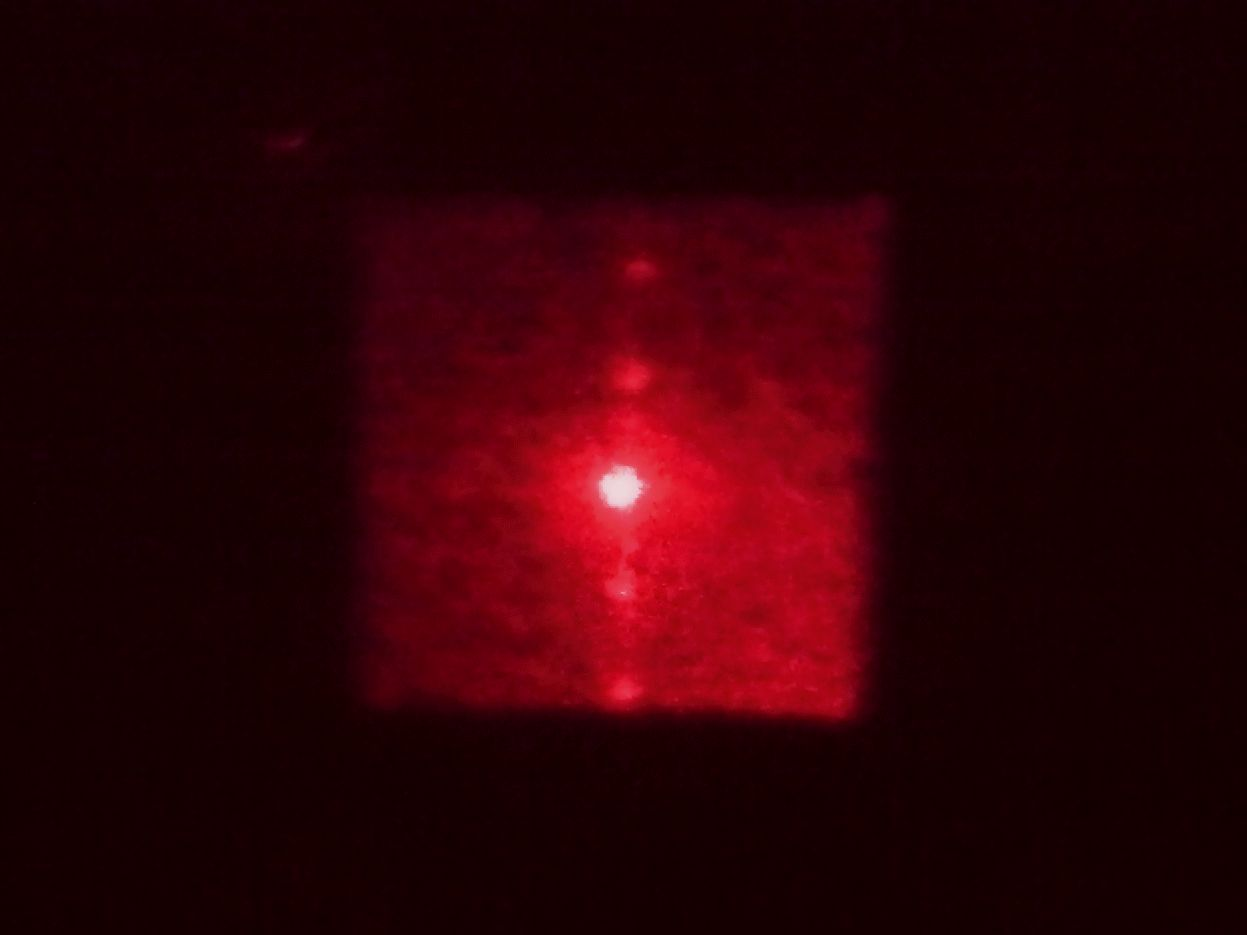
\includegraphics[width=\textwidth]{data/optics/06_Einstein_Dunkel_Beugung}
		\caption{Beugungsbild: Nebenmaximum}	 \label{fig:Einstein_dunkel_BG}
	\end{subfigure}
	\caption{Einstein-Portrait im Dunkelfeld}		\label{fig:Einstein_dunkel}
	\vspace{-5em}
\end{figure}




\newpage
\subsection{Transmissions-Elektronenmikroskop}

Unterfokus: Objekt unter Fokusebene (durch geringere Brennweite = stärkere Anregung der Spulen), im Bild 1. Saum dominierend hell (Fresnelsaum)

Überfokus analog

Diffractogramm: Fouriertrafo der Abbildung (aber wegen überlagerung mit ... schlechteres bild als im echten beugungsmodus)

Dunkler Ring im Diffractogramm normal, bei zweizähligem Astigmatismus wäre es zur Ellipse verzerrt, wird durch 2 Stigmatoren (Multipole) korrigiert


Aufnahmen:
Unter-, Über-, Fokus (F, Ü, U)
High resolution (mehrere bilder mit Netz ebenen)
Beugung (verdeckter Null Strahl zum Schutz der Kamera)
Bright, Dark Field

Diffractogramme nicht auf USB Stick dabei: freies Programm ImageJ, wahrscheinlich auch matlab (2D fft)

Meist nur eine Schar Netzebenen sichtbar (anstatt kariert) da die meisten Körner nicht in der fokusebene orientiert sind und somit nur eine Achse passt


Beugung: gewisse ringe auf unterschiedlichen Bildern an besten sichtbar, überlagern (entweder nur Messwerte oder Bilder)
Bei 340mm Kamera abstand (30000x Vergrößerung)
300mm Schirm Abstand (26500x Vergrößerung)

Brightfield: objektivblende lässt nur Hauptstrahl durch
Darkfield: ... nur Ausschnitt aus erstem beugungsRing durch
Zwei Bilder für unterschiedlichen Azimutwinkel --> unterschiedliche cluster leuchten auf (zwei verschiedene Orientierungen)




2. Probe
- convergent beam (Kreise mit gebogenem Linien, geben Aufschluss über dicke der probe)
- Beugung, gleiche Einstellungen wie bei der ersten probe

110 Orientierung
1-1+-1, -11+-1, ..., 002, ..., 004 Reflexe zu sehen



Bei der ersten probe
Träger = Kupfernetz + Kohlenstoff-Folie
Probe = kristallines Pulver (durch verdunsten des lösungsmittels gleichmäßig verteilt)

Erste probe Edelmetall (zu bestimmen, vermutlich Gold), zweite probe Si Kristall



